\providecommand{\reserveinserts}[1]{} % compatibility with the Wiley NJD v5 class
\makeatletter
\def\input@path{{wiley_template/}}
\makeatother

\documentclass[AMA,Times1COL]{WileyNJDv5}
\hypersetup{hidelinks}

\usepackage{booktabs}
\usepackage{amsmath,amssymb}
\usepackage{graphicx}
\usepackage{url}
\usepackage{placeins}
\usepackage{enumitem}
\usepackage{array}
\usepackage{longtable}
\usepackage[mathlines]{lineno}
\renewcommand\linenumberfont{\normalfont\scriptsize\sffamily}
\setlength\linenumbersep{10pt}

\graphicspath{{./}{figures/}{figures/si/}}

\setlist[itemize]{leftmargin=1.5em,itemsep=2pt,topsep=3pt}
\setlength{\parskip}{2.5pt}
\raggedbottom
\renewcommand{\thefigure}{S\arabic{figure}}
\renewcommand{\thetable}{S\arabic{table}}

\begin{document}

% ==================================================================
% TITLE PAGE
% ==================================================================

\begin{center}
\vspace*{0.12\textheight}

{\fontsize{11}{14}\selectfont\bfseries
Supporting Information for\par}

\vspace{8pt}

{\fontsize{18}{22}\selectfont\bfseries
Decision-Relevant Modelling of Extreme Demand for
Industrial Electricity Tariffs\par}

\vspace{14pt}

{\fontsize{10}{13}\selectfont
Mingyu Huang, Jiangweixi Wang, Zheng Gao, Yihang Yuan, Zhengjun Yang, and Huiqiong Li\par}

\vspace{4pt}

{\fontsize{9}{12}\selectfont
Department of Statistics and Data Science, School of Mathematics and Statistics, Yunnan University, Kunming 650500, China\par}

\vspace{10pt}

{\fontsize{9}{12}\selectfont
Applied Stochastic Models in Business and Industry\par}

{\fontsize{9}{12}\selectfont Correspondence: Huiqiong Li; \texttt{lihuiqiong@ynu.edu.cn}\par}

\end{center}

\vfill
\clearpage
\resetlinenumber[1]\linenumbers


% ==================================================================
% APPENDIX S1
% ==================================================================

\section*{Appendix S1. Supplementary methods, derivations, and analyses}

This Supporting Information provides technical derivations,
implementation details, complete supplementary summaries, robustness
analyses, and external predictive analyses referenced in the main
article. The primary controlled experiment compares five predictive
constructions. TAIL and EVENT-EMP use event-level histories, whereas
GEV, KDE, and EMP use the corresponding monthly maxima. The primary controlled
experiment contains 10,000 independent 24-month histories and nine
prespecified tariff cells, giving 450,000
history--method--cell decisions. Supplementary recovery, stress,
physical-clipping, and physical-misspecification experiments are
separate experiments and retain their own stated analysis units.

Throughout, \(M\geq0\) denotes monthly maximum demand,
\(F\) its distribution,
\[
\mu_F=\mathbb E_F[M],
\qquad
H_F(t)=\mathbb E_F[(M-t)_+].
\]
The reference capacity is \(S\), the contract level is \(D\),
the contract-threshold multiplier is \(\alpha\), the lower contract
fraction is \(\delta\), and the exceedance-charge multiplier is
\(\kappa\). Optimized mode values are denoted by \(V_F(m)\),
the oracle value by \(V_F^\ast\), oracle mode separation by
\(\gamma_F\), and the maximum mode-value perturbation by \(e_V\).
The retrospective stability ratio is
\[
d_{MV}=\frac{2e_V}{\gamma_F}.
\]
For a selected full action \(\widehat a\), regret is
\[
R_F(\widehat a)
=
C_F(\widehat a)-V_F^\ast.
\]


% ==================================================================
% S1.1
% ==================================================================

\subsection*{S1.1 Supplementary tariff identities and decision-stability details}

The main article gives the tariff functionals and the principal
decision-stability results. This subsection records only the
atom-aware and boundary details used by the implementation.

For the contract objective
\[
\phi_F(D)
=
D+\kappa H_F(\alpha D),
\qquad
D\in[\delta S,S],
\]
the stop-loss functional has one-sided derivatives
\[
H'_{F,+}(t)
=
-\Pr_F(M>t),
\qquad
H'_{F,-}(t)
=
-\Pr_F(M\geq t).
\]
Consequently,
\[
\partial\phi_F(D)
=
\left[
1-\kappa\alpha\Pr_F(M\geq\alpha D),
\;
1-\kappa\alpha\Pr_F(M>\alpha D)
\right].
\]
For an interior optimizer this gives
\[
\Pr_F(M>\alpha D^\ast)
\leq
\frac{1}{\kappa\alpha}
\leq
\Pr_F(M\geq\alpha D^\ast).
\]
Writing
\[
p^\ast
=
1-\frac{1}{\kappa\alpha},
\]
\(\alpha D^\ast\) is therefore a generalized \(p^\ast\)-quantile.
The feasible-boundary cases are handled by restricting the generalized
quantile solution to
\[
D\in[\delta S,S].
\]

\paragraph*{Mode stability and demand-scale radii.}
For a unique oracle tariff mode $m_F^\ast$, define, for each
$m\neq m_F^\ast$,
\[
\gamma_{F,m}=V_F(m)-V_F(m_F^\ast),
\]
and, for every $j\in\mathcal M$,
\[
e_j=\left|V_{\widehat F}(j)-V_F(j)\right|.
\]
The pairwise sufficient condition is
\[
e_m+e_{m_F^\ast}<\gamma_{F,m}
\qquad
\text{for every }m\neq m_F^\ast.
\]
With
\[
e_V=\max_{j\in\mathcal M}e_j,
\qquad
\gamma_F=\min_{m\neq m_F^\ast}\gamma_{F,m},
\]
the scalar condition
\[
d_{MV}=\frac{2e_V}{\gamma_F}<1
\]
is a simpler conservative sufficient certificate. Both conditions
use oracle quantities and are retrospective diagnostics in the
controlled experiment.

For the Wasserstein representation, let
\[
L_{\mathrm{cap}}=0,\qquad
L_{\mathrm{act}}=r_d,\qquad
L_{\mathrm{con}}=r_d\kappa.
\]
The corresponding analytic demand-scale radii are
\[
\rho_F^{\mathrm{pair}}
=\min_{m\neq m_F^\ast}
\frac{\gamma_{F,m}}{L_m+L_{m_F^\ast}},
\qquad
\rho_F=\frac{\gamma_F}{2L},
\qquad
L=r_d\max\{1,\kappa\}.
\]
Table~\ref{tab:analytic-demand-radii} reports the primary tariff
geometry and these oracle-dependent radii. They contain neither a
numerical integration allowance nor a solver allowance.

\paragraph*{Full-action loss.}
The exact regret decomposition separates mode-selection loss from
within-mode excess. The latter is identically zero for actual demand
and capacity. Only contract demand can have nonzero within-mode
excess. If contract demand is both oracle optimal and selected, and
$\widehat D$ exactly minimizes the fitted contract objective, then
\[
R_F\!\left(a_{\mathrm{con}}(\widehat D)\right)
\leq
2r_d\kappa\,\Delta_H(F,\widehat F),
\]
where
\[
\Delta_H(F,\widehat F)
=\sup_{D\in\mathcal D_S}
\left|H_{\widehat F}(\alpha D)-H_F(\alpha D)\right|.
\]

As an implementation check, the exact regret decomposition was
verified on all $450{,}000$ primary decision rows, with no
failures; the maximum absolute residual was
$7.45\times10^{-9}$ CNY/month.


% ==================================================================
% S1.2
% ==================================================================

\subsection*{S1.2 Analytic oracle and deterministic numerical evaluation}

The controlled data-generating mechanism admits an analytic
monthly-maximum distribution. In each month, 200 bounded bulk events
are generated as
\[
X^{(b)}
=
45{,}000+35{,}000\,B,
\qquad
B\sim\operatorname{Beta}(8,2),
\]
and an independent number
\[
N\sim\operatorname{Poisson}(30)
\]
of tail events is generated as
\[
X^{(t)}
=
80{,}000+Y,
\qquad
Y\sim\operatorname{GPD}(\xi=0.15,\sigma=12{,}000).
\]
The monthly maximum \(M\) is the maximum over the bulk and tail
events.

Let
\[
L=45{,}000,
\qquad
u_0=80{,}000,
\qquad
\lambda=30,
\]
and let \(F_B\) denote the
\(\operatorname{Beta}(8,2)\) distribution function. The exact
monthly-maximum CDF is
\[
F_M(x)
=
\begin{cases}
0,
&
x<L,
\\[4pt]
\exp(-\lambda)
\left[
F_B\!\left(
\dfrac{x-L}{u_0-L}
\right)
\right]^{200},
&
L\leq x<u_0,
\\[10pt]
\displaystyle
\exp\left[
-\lambda
\left\{
1+\xi\frac{x-u_0}{\sigma}
\right\}^{-1/\xi}
\right],
&
x\geq u_0.
\end{cases}
\]

The resulting oracle quantities are
\[
\mu_F
=
148{,}235.371489\ {\rm kW},
\]
\[
q_{0.99}
=
265{,}663.010007\ {\rm kW},
\]
and
\[
q_{0.999}
=
375{,}513.529996\ {\rm kW}.
\]

The oracle mean and stop-loss functionals are evaluated from
\[
\mu_F
=
\int_0^\infty
\{1-F_M(x)\}\,dx
\]
and
\[
H_F(t)
=
\int_t^\infty
\{1-F_M(x)\}\,dx.
\]
High quantiles are obtained from the analytic distribution. The same
oracle law therefore determines the reference capacity
\[
S=\frac{\mu_F}{u},
\]
the tariff-mode values, the optimized contract level, the unique
oracle mode where applicable, and the oracle mode separation
\(\gamma_F\).

Final fitted-law evaluation likewise avoids a common predictive
Monte Carlo layer between \(\widehat F\) and the tariff functionals.
Finite discrete distributions use exact sums. The nonnegative
Gaussian KDE uses analytic Gaussian-mixture expressions for its mean
and stop-loss function. The fitted tail-process and
nonnegative-conditioned GEV constructions use deterministic
one-dimensional integration where required, and continuous quantiles
are obtained by direct inversion or deterministic bracketed root
finding.

The deterministic numerical layer was independently checked in
55 numerical comparisons. The maximum relative discrepancy was
approximately
\[
1.283\times10^{-11}.
\]
No Monte Carlo approximation to the oracle is used in the reported
controlled experiment.


% ==================================================================
% S1.3
% ==================================================================

\subsection*{S1.3 Predictive-construction implementation}

The five primary predictive constructions are organized by their
information source. TAIL and EVENT-EMP use event-level observations.
GEV, KDE, and EMP use the 24 observed monthly maxima. This distinction
is retained because comparisons across the two groups combine
differences in information resolution and distributional construction,
whereas TAIL versus EVENT-EMP and comparisons within
GEV/KDE/EMP provide same-broad-information contrasts.


\subsubsection*{Event-level constructions}

\paragraph*{TAIL.}

TAIL receives event-level maxima with month identifiers. Specification
selection uses the first 19 months for candidate fitting and the final
five months for internal predictive validation. Candidate thresholds
are the empirical event-level quantiles
\[
0.90,\qquad
0.925,\qquad
0.95,\qquad
0.975.
\]
For a candidate numerical threshold \(u\), exceedances are strict:
only observations \(Z>u\) enter the excess sample
\[
Y=Z-u.
\]
The excess law is fitted by GPD maximum likelihood with location fixed
at zero.

Monthly exceedance counts are formed over all fitting months,
including months with zero exceedances. If \(\bar N\) and \(s_N^2\)
denote the empirical monthly count mean and variance, the count law is
Poisson when the variance-to-mean ratio is at most 1.2 or when the
empirical mean is nonpositive. Otherwise the negative-binomial
method-of-moments parameters are
\[
r
=
\frac{\bar N^2}{s_N^2-\bar N},
\qquad
p
=
\frac{r}{r+\bar N}.
\]
The corresponding probability-generating functions are
\[
P_N(z)
=
\exp\{\lambda(z-1)\}
\]
for the Poisson case and
\[
P_N(z)
=
\left[
\frac{p}{1-(1-p)z}
\right]^r
\]
for the negative-binomial case.

Candidate screening requires at least 100 strict exceedances.
Shape stability is assessed from 50 nonparametric excess-sample
bootstrap fits, with at least 40 successful fits required and the
resulting 95\% shape-interval width not exceeding 0.8. The
success requirement is 80\% of the configured replicate count,
with at least 40 fits in the primary experiment. The
probability-transformed fitted tail must satisfy a
Kolmogorov--Smirnov \(p\)-value threshold of 0.01. For a negative-shape
candidate, the natural finite endpoint
\[
e_u
=
u-\frac{\widehat\sigma_u}{\widehat\xi}
\]
must satisfy
\[
e_u\geq \max_i X_i-10^{-9},
\]
where \(X_i\) are the fitting-period event maxima in kW. Candidate
fits must have a finite validation score and satisfy
\[
\widehat\xi<1,
\]
which ensures a finite first moment.

For each fitted candidate, we simulate \(m=2{,}000\) monthly maxima
\(Z_1,\ldots,Z_m\) on the fitted candidate's natural support, without
artificial upper clipping, and estimate their density with a Gaussian
kernel:
\[
\widehat f_m(y)=\frac{1}{mh}\sum_{j=1}^{m}
\phi\!\left(\frac{y-Z_j}{h}\right),
\qquad h=s_Zm^{-1/5},
\]
where \(\phi\) is the standard normal density and \(s_Z\) is the
sample standard deviation with denominator \(m-1\). This is Scott's
bandwidth as implemented by \texttt{scipy.stats.gaussian\_kde}.
For the five held-out monthly maxima \(Y_1,\ldots,Y_5\), the score is
\[
\ell_{\rm val}=\frac{1}{5}\sum_{t=1}^{5}
\log\!\left\{\max\bigl(\widehat f_m(Y_t),\epsilon_{\rm tiny}\bigr)\right\},
\qquad \epsilon_{\rm tiny}=2.2250738585072014\times10^{-308}.
\]
A numerically constant predictive sample has an undefined score and
is excluded. If \(\mathcal P\) denotes the candidates that pass the
screening and finite-mean conditions, the selection score is
\[
\ell_{\rm val}
-
0.10
\left|
\widehat\xi
-
\operatorname{median}_{j\in\mathcal P}
(\widehat\xi_j)
\right|.
\]
An exact tie is resolved toward the lower threshold quantile.

The 19/5 split is used only for specification selection. After the
numerical threshold is selected, that threshold is held fixed and the
GPD parameters, exceedance-count law, and empirical subthreshold
component are reconstructed using all 24 months.

If no admissible finite-mean primary candidate is available but an
eligible threshold has at least 50 exceedances, the procedure uses an
exponential-tail fallback with
\[
\xi=0
\]
and scale equal to the corresponding mean excess. If no such threshold
is available, the monthly-maxima empirical distribution is used.
An invalid all-history GPD refit likewise invokes the prescribed
fallback branch.

For a final primary TAIL fit, let \(F_0\) denote the empirical CDF of
the subthreshold monthly-maximum component, let \(G_u\) denote the
fitted GPD excess CDF, and let \(P_N\) denote the fitted exceedance-count
probability-generating function. The monthly-maximum CDF is
\[
\widehat F_{\rm TAIL}(x)
=
\begin{cases}
F_0(x)P_N(0),
&
x<u,
\\[4pt]
P_N\!\left\{G_u(x-u)\right\},
&
x\geq u.
\end{cases}
\]
The final mean is evaluated as
\[
\mu_{\widehat F_{\rm TAIL}}
=
H_{\widehat F_{\rm TAIL}}(0),
\]
the stop-loss function is obtained by deterministic integration of the
fitted survival function, and continuous quantiles are obtained by
deterministic inversion. Thus the simulation used for internal
candidate validation is not reused as the final representation of the
tariff-relevant functionals.



\paragraph*{EVENT-EMP.}

EVENT-EMP uses the same event-level history as TAIL but imposes no
threshold or parametric tail/count model. Let \(\widehat G_E\) denote
the pooled empirical CDF of all event-level maxima in the 24-month
history, and let \(N_m\) denote the observed total event count in
month \(m\). The induced monthly-maximum CDF is
\[
\widehat F_{\rm EE}(x)
=
\frac{1}{24}
\sum_{m=1}^{24}
\widehat G_E(x)^{N_m}.
\]
This is a finite discrete distribution. Its probability masses are the
jumps of \(\widehat F_{\rm EE}\); its mean and stop-loss function are
evaluated exactly by finite sums, and its quantiles use the discrete
left inverse. There is no dedicated fallback branch.

TAIL and EVENT-EMP therefore use the same broad event-level
information source but different distributional constructions. TAIL
adds threshold selection, a parametric excess law and a fitted
exceedance-count law, whereas EVENT-EMP combines a pooled empirical
event distribution with the empirical distribution of observed
monthly event counts.


\subsubsection*{Monthly-maxima constructions}

\paragraph*{GEV.}

The controlled-experiment GEV construction uses the 24 observed
monthly maxima. It is fitted using L-moments/probability-weighted
moments rather than maximum likelihood. L-skewness is inverted
deterministically for the EVT shape parameter within
\[
[-0.90,0.90],
\]
and the location and scale parameters follow from the associated
L-moment equations.

A successful raw GEV fit is conditioned on the nonnegative part of its
model-implied natural support. If more than 1\% of the raw fitted GEV
probability lies below zero, or if the L-moment fit or resulting
parameters are invalid, the procedure uses the empirical
monthly-maxima distribution. Successful parametric fits satisfy the
finite-mean requirement. When the fitted EVT shape is negative, its
model-implied finite upper endpoint is retained; otherwise the upper
support is unbounded.

The conditioned GEV mean and stop-loss function are evaluated
deterministically over this support, using one-dimensional integration
where required. Quantiles use the conditioned inverse distribution.
This GEV construction is distinct from the K-GEV procedure used in the
external manufacturing-load analysis.


\paragraph*{KDE.}

KDE is fitted to the 24 monthly maxima
\(M_1,\ldots,M_n\), with \(n=24\), using bandwidth
\[
h
=
1.06\,s\,n^{-1/5},
\]
where \(s\) is the sample standard deviation. The Gaussian mixture is
conditioned on nonnegative demand. If
\[
\widetilde F(x)
=
\frac{1}{n}
\sum_{i=1}^{n}
\Phi\left(\frac{x-M_i}{h}\right)
\]
denotes the unconditioned Gaussian-mixture CDF and
\[
Z_+
=
1-\widetilde F(0),
\]
then
\[
\widehat F_{\rm KDE}(x)
=
\begin{cases}
0,
&
x<0,
\\[3pt]
\dfrac{\widetilde F(x)-\widetilde F(0)}{Z_+},
&
x\geq0.
\end{cases}
\]

For \(t\geq0\), its stop-loss function is
\[
H_{\widehat F_{\rm KDE}}(t)
=
\frac{1}{nZ_+}
\sum_{i=1}^{n}
\left[
(M_i-t)
\Phi\left(\frac{M_i-t}{h}\right)
+
h\phi\left(\frac{t-M_i}{h}\right)
\right],
\]
where \(\Phi\) and \(\phi\) are the standard normal CDF and PDF.
Setting \(t=0\) gives the mean. Quantiles are obtained by deterministic
inversion of the conditioned mixture CDF. If fewer than two
observations are available or the observed variability is numerically
degenerate, the implementation uses the empirical distribution.


\paragraph*{EMP.}

EMP assigns empirical probability to the 24 observed monthly maxima,
with duplicate support values aggregated. For support points \(x_j\)
with empirical probabilities \(p_j\),
\[
\mu_{\widehat F_{\rm EMP}}
=
\sum_jp_jx_j,
\]
and
\[
H_{\widehat F_{\rm EMP}}(t)
=
\sum_jp_j(x_j-t)_+.
\]
Quantiles use the empirical left inverse. No predictive-bootstrap layer
is introduced into the final tariff-functional evaluation.


% ==================================================================
% S1.4
% ==================================================================

\subsection*{S1.4 From predictive laws to tariff actions}

Every fitted predictive law is passed through the same tariff-action
map. For the evaluated policies, \(\kappa\alpha>1\), and the interior
contract probability is
\[
p^\ast
=
1-\frac{1}{\kappa\alpha}.
\]
For a fitted law \(\widehat F\), define the left generalized quantile
\[
\widehat q_p
=
\inf\{x:\widehat F(x)\geq p\}.
\]
The final contract level is
\[
\widehat D
=
\operatorname{clip}
\left(
\frac{\widehat q_{p^\ast}}{\alpha},
\delta S,
S
\right).
\]
Thus lower and upper boundary solutions are handled directly through
the feasible interval. No predictive Monte Carlo candidate search or
local order-statistic candidate set is used.

The fitted optimized tariff-mode values are
\[
V_{\widehat F}(\operatorname{cap})
=
r_cS,
\]
\[
V_{\widehat F}(\operatorname{act})
=
r_d\mu_{\widehat F},
\]
and
\[
V_{\widehat F}(\operatorname{con})
=
r_d
\left\{
\widehat D
+
\kappa
H_{\widehat F}(\alpha\widehat D)
\right\}.
\]
The selected tariff mode minimizes these deterministic mode values.
Exact mode-value ties are resolved by the fixed lexicographic order
\[
\operatorname{actual\ demand}
\;\prec\;
\operatorname{capacity}
\;\prec\;
\operatorname{contract\ demand}.
\]

For discrete predictive laws, the left-quantile convention fixes the
generalized-quantile representative. For continuous laws, quantiles
are obtained directly or by deterministic root inversion.

Although
\[
V_F(\operatorname{cap})=r_cS
\]
does not itself contain a distributional functional, selection of the
capacity mode depends on its comparison with the estimated
actual-demand and contract-demand mode values. Under contract demand,
the complete action additionally contains \(D\); consequently,
tariff-mode correctness and full-action optimality are separate
endpoints.


% ==================================================================
% S1.5
% ==================================================================

% ==================================================================
% S1.5
% ==================================================================

\subsection*{S1.5 Primary comparisons and high-$p^*$ tariff stress}

The complete nine-cell primary summaries, mode-versus-within-contract
regret decomposition, and core paired contrasts are reported in the main
article. Supplementary Table~S12 gives all ten region-specific paired
comparisons for the final 10,000-history primary run. It is a complete
reference table; the ten contrasts are not treated as one confirmatory
family.

The high-$p^*$ stress analysis evaluates three target quantiles over ten
utilization cells, using 10,000 histories and five predictive methods.
Figure~\ref{fig:final-figures1} and Table~\ref{tab:si-high-pstar}
report the history-level regret distributions, exact-zero-regret rates,
and same-information paired comparisons. This stress design is separate
from the nine-cell primary analysis.

% ==================================================================
% S1.6
% ==================================================================

\subsection*{S1.6 Functional-error associations and certificate-conditioned loss}

Figure~\ref{fig:final-figures2} summarizes the within-method association
of regret with absolute mean, stop-loss, and $q_{0.99}$ relative errors,
and the concentration of regret among the largest-loss decisions.
Table~\ref{tab:final-si-7} reports the paired functional-correlation
contrasts with simultaneous max-$|T|$ intervals. Table~\ref{tab:si-certificate}
reports within-contract loss among decisions stratified by certificate
status. The certificate is a sufficient condition; observations outside
the certified set are not classified as violations.

% ==================================================================
% S1.7
% ==================================================================

\subsection*{S1.7 Numerical bounds and fitting-support sensitivity}

The theoretical sufficient conditions in the main article are
summarized separately from their numerical implementation. The
numerical audit uses upper constructions for the relevant distributional
perturbations and a common numerical full-action solver allowance.
For the primitive-action perturbation, the reported numerical upper
quantity is
\[
\varepsilon_{\rm num}
=\max\left\{
r_d\left|\widehat\mu-\mu_F\right|,
\;r_d\kappa\Delta_{H,\rm upper}
\right\}.
\]
It is a numerical upper bound on primitive-action perturbation, not the
mode-value error $e_V$ and not an exact analytic supremum. The
feasible-threshold stop-loss quantity uses a direct 513-node estimate
and a numerical upper allowance based on the monotone-CDF envelope and
half-grid spacing; it is a numerical upper bound on the feasible
stop-loss perturbation.

The primitive numerical sufficient-condition check is
\[
2\varepsilon_{\rm num}+\zeta_{\rm full,num}<\gamma_F.
\]
For each non-oracle competitor $m$, the direct
contrast-Wasserstein check is
\[
K_{m,m_F^\ast}W_{1,\rm upper}
+\zeta_{\rm full,num}<\gamma_{F,m},
\]
where $K_{\mathrm{cap},\mathrm{act}}=r_d$,
$K_{\mathrm{cap},\mathrm{con}}=r_d\kappa$, and
$K_{\mathrm{act},\mathrm{con}}=r_d\max\{1,|1-\kappa|\}$.
The mode-wise pairwise Wasserstein comparator instead uses
\[
(L_m+L_{m_F^\ast})W_{1,\rm upper}
+\zeta_{\rm full,num}<\gamma_{F,m},
\]
for every non-oracle competitor, and the uniform Wasserstein check is
\[
2L W_{1,\rm upper}+\zeta_{\rm full,num}<\gamma_F,
\qquad L=r_d\max\{1,\kappa\}.
\]
The numerical Wasserstein upper quantity is based on CDF bounds; the
point estimates reported in Table~\ref{tab:final-si-6} use numerical
quadrature. The solver allowance and distributional numerical quantities are
floating-point implementation bounds without directed-rounding or
interval-arithmetic guarantees. Table~\ref{tab:numerical-sufficient-condition-audit}
reports the observed implementation-audit results: the primitive-
perturbation check was satisfied by $26{,}975/450{,}000$
($5.994444\%$); the direct contrast-Wasserstein check by
$57{,}501/450{,}000$ ($12.778000\%$); the mode-wise
pairwise-Wasserstein check by $26{,}393/450{,}000$
($5.865111\%$); and the uniform-Wasserstein check by
$5{,}329/450{,}000$ ($1.184222\%$). No observed mode-selection
violations occurred among rows satisfying any of these four numerical
checks.

\paragraph*{Fitting-support sensitivity.}
The primary controlled analysis evaluates each fitted law on the
estimator-specific support described in Section S1.3. To assess
sensitivity to finite fitting bounds, a paired analysis uses the first
\(1{,}000\) primary histories and the same nine tariff cells. Three
training-derived upper bounds are considered:
\[
B_{\rm tr}^{(10)}
=
10\max_{1\leq m\leq24} M_m,
\qquad
B_{\rm tr}^{(20)}
=
20\max_{1\leq m\leq24} M_m,
\qquad
B_{\rm tr}^{(50)}
=
50\max_{1\leq m\leq24} M_m,
\]
where \(M_1,\ldots,M_{24}\) are the observed training monthly maxima.
Because the data-generating distribution is known in the controlled
experiment, the sensitivity analysis also includes the
oracle-referenced diagnostic bound
\[
B_{\rm or}
=
10q_{0.999}.
\]
This diagnostic specification is used only in the sensitivity
analysis. The same histories and tariff cells are retained under every
support rule. The support treatment affects the TAIL and GEV
constructions; EVENT-EMP, KDE, and EMP are unchanged by construction.

Panels (d--f) of Figure~\ref{fig:final-figures3} summarize the paired
support-policy comparisons relative to the primary specification.
Panels (d) and (e) show cellwise paired mean changes in regret for TAIL
and GEV, respectively, with one paired Monte Carlo standard error, and
panel (f) shows the percentage of TAIL tariff-mode decisions that
change. Table~\ref{tab:final-si-11} reports, for both TAIL and GEV, the
paired mean regret change, its paired standard error, and the percentage
of changed tariff-mode decisions in each tariff cell. Across the
displayed support rules and cells, the changed-mode percentage does not
exceed \(0.20\%\) for TAIL or \(0.40\%\) for GEV. The largest absolute
cellwise paired mean-regret changes are \(0.062\) and \(0.726\) thousand
CNY/month for TAIL and GEV, respectively.

% ==================================================================
% S1.8
% ==================================================================

\subsection*{S1.8 Parameter recovery and threshold-fixed bootstrap interval coverage}


The parameter-recovery experiment is separate from the 10,000-history
primary comparison. It uses 200 histories at each of 12, 24, and
60 months under a Poisson--GPD mechanism with generating threshold
\(80{,}000\) kW,
\[
\xi=0.15,
\qquad
\sigma=12{,}000\ {\rm kW},
\]
and a Poisson rate of 30 tail events per month.

The threshold continues to be selected by the fitted procedure rather
than fixed at the generating threshold. Scale recovery is therefore
evaluated relative to the threshold-specific scale implied by GPD
threshold stability.

The mean absolute errors of the fitted shape parameter are
\[
0.0699,\qquad
0.0578,\qquad
0.0343
\]
for 12, 24, and 60 months, respectively. Figure S4 reports the
complete shape-error, relative-scale-error, and relative-\(q_{0.99}\)
error distributions.

\FloatBarrier

For each history of length \(n\) months, we construct nominal 95\%
nonparametric percentile intervals for the GPD shape and scale.
The selected threshold \(\widehat v\) is held fixed. We draw 100
bootstrap samples with replacement from the excesses in the first
\(\lfloor0.8n\rfloor\) months, preserving the excess count, and fit
a GPD with location fixed at zero to each sample. The interval
endpoints are the 2.5th and 97.5th percentiles of the valid parameter
estimates; at least 75 finite fits with positive scale are required.
Shape coverage is evaluated against \(\xi=0.15\), and scale coverage
against \(\sigma(\widehat v)=12000+0.15(\widehat v-80000)\).
Table~S10 reports coverage across 200 histories and 95\%
Clopper--Pearson intervals for its Monte Carlo uncertainty.
Thresholds vary across histories and remain fixed within each
bootstrap calculation.


% ==================================================================
% S1.9
% ==================================================================

\subsection*{S1.9 Physical clipping identity and sensitivity}

Let latent event-level demand values be \(X_i\), and let physical
clipping operate at level \(c\). Clipping commutes with maximization:
\[
\min\left(\max_iX_i,c\right)
=
\max_i\min(X_i,c).
\]
Thus clipping individual events before monthly maximization yields the
same clipped monthly maximum as clipping the corresponding original
monthly maximum.

Let
\[
M_c=\min(M,c)
\]
and let \(F_c\) denote its distribution. Pointwise,
\[
M_c=M-(M-c)_+,
\]
so
\[
\mathbb E[M_c]
=
\mathbb E[M]-H_F(c).
\]
For every \(t\leq c\),
\[
(\min(M,c)-t)_+
=
(M-t)_+-(M-c)_+,
\]
and therefore
\[
H_{F_c}(t)
=
H_F(t)-H_F(c),
\qquad
t\leq c.
\]
For \(t\geq c\),
\[
H_{F_c}(t)=0.
\]
The equality case \(t=c\) is included in the first identity.

The clipping experiment uses four physical regimes:
\[
\begin{aligned}
\mathrm{UNCAPPED}:&
\quad c=10q_{0.999},
\\
\mathrm{DISTANT}:&
\quad c=\frac{q_{0.999}}{0.85},
\\
\mathrm{Q999}:&
\quad c=q_{0.999},
\\
\mathrm{BINDING}:&
\quad c=\frac{q_{0.999}}{1.25}.
\end{aligned}
\]
``UNCAPPED'' is an experimental label for a distant finite physical
clipping level. Its value \(c=10q_{0.999}\) defines a clipping regime
only in this robustness experiment. The clipping level \(c\) is
applied to generated demand and is distinct from the fitted-law support
treatment used in the primary controlled analysis.

The experiment uses 12- and 24-month histories,
\[
u\in\{0.62,0.63,0.64\},
\]
and 200 histories for each
history-length--clipping--utilization setting. TAIL, KDE, EMP, and the
robustness-only GATE selector are retained. In this experiment, normalized regret is one-month regret divided by
one monthly capacity fee;
it is distinct from the primary normalized regret \(R_F/V_F^\ast\).

GATE selects TAIL when its fit status is \texttt{PASS}, the fraction
of reconstructed maxima exceeding the support bound is at most 0.01,
and two consecutive available threshold candidates pass screening
with shape estimates of the same sign. Candidates are ordered by
their threshold quantiles \(0.90,0.925,0.95,0.975\); the qualifying
pair need not include the threshold ultimately selected by TAIL.
Each member must have at least 100 exceedances, a nominal 95\%
bootstrap shape-interval width at most 0.8, a uniform-transform KS
\(p\)-value at least 0.01, and a compatible endpoint when its shape
is negative, as defined in S1.3. GATE otherwise selects KDE.
Shape-width screening uses 50 bootstrap resamples here and 500 in
the physical-pipeline experiment in S1.10, with at least 80\% valid refits.
The support bound is the clipping level \(c\) here and 120 MW in
S1.10. Two zero shape estimates count as having the same sign.

Figure S5 reports paired TAIL-minus-baseline ECDFs after averaging the
three utilization cells within history. Negative values favour TAIL.
ECDFs are used because the interquartile ranges of all 16 plotted
contrast groups are zero and boxplots would obscure their nonzero
tails.

\FloatBarrier



% ==================================================================
% S1.10
% ==================================================================

\subsection*{S1.10 Physical-pipeline stress at $\alpha=1.20$}

The physical-pipeline experiment evaluates high-amplitude,
high-frequency, and clustered-event mechanisms at $\alpha=1.20$. Each
method, training length, and tariff cell is evaluated on 200 paired
histories, for 72,800 decision records. Figure~\ref{fig:final-figures6}
and Table~\ref{tab:si-s6-updated} report the distributional and
cell-aggregated results.

\subsection*{S1.11 Joint negative-binomial--Weibull challenge}

The joint misspecification challenge combines a negative-binomial event
count with Weibull exceedances. Figure~\ref{fig:final-figures7} shows the
cellwise distribution of regret across the actual, contract, and
capacity oracle regions. Table~\ref{tab:final-si-4} gives the complete
cell-by-method results, and Table~\ref{tab:final-si-5} gives the full
regional paired contrasts. This experiment assesses a joint count and
severity misspecification and is not used as a replacement for the
physical-pipeline experiment above.

% ==================================================================
% S1.12
% ==================================================================

\subsection*{S1.12 Crossed tariff geometry without an artificial upper fitting bound}

The crossed-grid analysis evaluates five methods over 19 utilization
values at $\alpha\in\{1.05,1.10,1.15,1.20\}$ using 1,000 shared
histories, for 380,000 decisions. Figure~\ref{fig:crossed-grid-all-methods}
shows mean normalized full-action regret and oracle-mode accuracy. The
curves connect discrete evaluated tariff cells for visual comparison;
no interpolation or invariant within-region ranking is implied.

% ==================================================================
% S1.13
% ==================================================================

\subsection*{S1.13 External manufacturing-load design and predictive constructions}

The external analysis uses the public South Korean
manufacturing-factory electricity dataset described by Lee, Baek and
Kim~\cite{Lee2022} and its associated Figshare release
\cite{LeeFigshare}. The source contains one-minute electricity-demand
records for 10 manufacturing facilities from March through September
2019. All 10 facilities are retained for descriptive upper-tail
summaries, whereas eight factories satisfy the completeness
requirements for formal rolling predictive evaluation.

The formal series is reconstructed using fixed, non-overlapping
15-minute averages. Timestamps must be valid, duplicate timestamps are
resolved before reconstruction, and demand values must be numeric and
nonnegative. A reconstructed 15-minute window is retained only when
all 15 constituent one-minute observations are available; no
imputation is applied to the primary tail series. A factory-month is
eligible when at least 95\% of its reconstructed windows are valid.

The primary natural-tail analysis removes documented demand-response
intervals and the subsequent 60-minute rebound period. The
all-observations sensitivity analysis retains these intervals while
otherwise preserving the same rolling evaluation.

Four expanding-window forecast origins are used:
\[
\begin{aligned}
\text{March--May}&\rightarrow\text{June},\\
\text{March--June}&\rightarrow\text{July},\\
\text{March--July}&\rightarrow\text{August},\\
\text{March--August}&\rightarrow\text{September}.
\end{aligned}
\]
For origin \(o\), let \(T_o\) denote its set of training months and
let \(M_{o,m}\) denote the maximum reconstructed 15-minute load in
training month \(m\). The training-derived normalization is
\[
s_o
=
\frac{1}{|T_o|}
\sum_{m\in T_o}
M_{o,m}.
\]
The same scale is applied to the corresponding final training series
and test month.

For candidate tail specifications, model selection is internal to the
training window. Each available training month is held out in turn,
the candidate is fitted using the remaining training months, and its
predictive score is evaluated on the held-out training month.
Candidate scores are averaged across these
leave-one-training-month-out folds. Within each internal fold, the
normalization is recomputed using only the fold-fitting months and is
then applied to its held-out training month. The test month is never
used for specification selection. After candidate selection, the
chosen specification is refitted using all training months before the
test-month maximum is scored. The recorded internal-validation
registry contains 3,456 candidate-fold records.

The formal external evaluation contains seven predictive
constructions:
K-BLOCK, K-EMP, K-GEV, K-GTAIL, K-KDE, K-POINT, and K-UGPD.
With eight eligible factories and four forecast origins, each method
contributes 32 factory--origin predictions, giving 224
method--factory--origin records across the seven methods.

\paragraph*{K-EMP.}

K-EMP uses the normalized training monthly maxima. Unlike controlled
EMP, whose downstream tariff functionals are evaluated exactly as a
finite discrete law, the external K-EMP scoring representation uses
50,000 bootstrap predictive draws from the empirical training
monthly-maximum distribution at each rolling origin.

\paragraph*{K-KDE.}

K-KDE uses the same normalized training monthly maxima. Its Gaussian
residual/kernel representation uses
\[
h=1.06\,s\,n^{-1/5}.
\]
Negative proposals are rejected, and the final external scoring
representation contains 50,000 predictive draws. This draw-based
external representation is distinct from the deterministic
nonnegative Gaussian-mixture evaluation used by controlled KDE.

\paragraph*{K-BLOCK.}

K-BLOCK is a high-frequency non-EVT reference based on the
reconstructed normalized 15-minute training series. A 24-hour block
contains 96 consecutive 15-minute windows. The implementation first
forms moving 96-window maxima within each training month, pools these
complete-block maxima over the training months, and resamples them with
replacement. Only blocks containing 96 observations at consecutive
15-minute timestamps are eligible. For a target month containing $d$
days, the procedure samples $d$ eligible 24-hour block maxima with
replacement and takes their maximum as one synthetic monthly maximum.
The external predictive scoring layer uses 50,000 such draws. Thus the
implemented procedure resamples complete 24-hour block maxima rather
than raw 15-minute observations.
Across all 32 factory--origin fits, the 402,570 eligible blocks had
consecutive 15-minute timestamps. These verified block sets were used
for K-BLOCK prediction.

\paragraph*{K-POINT.}

K-POINT is a degenerate predictive reference concentrated at the mean
of the normalized training monthly maxima.

\paragraph*{K-GTAIL.}

K-GTAIL is a runs-declustered peaks-over-threshold construction fitted
to the normalized fixed-15 training series. Candidate threshold
quantiles are
\[
\{0.90,0.925,0.95,0.975\},
\]
and candidate run lengths are
\[
\{30,60,120\}\ {\rm minutes}.
\]
Exceedances are strict. Exceedances separated by no more than the
candidate run length belong to the same run cluster, and each cluster
is represented by its maximum excess. GPD excesses are fitted by
maximum likelihood with location fixed at zero.

Every threshold--run candidate is evaluated through the
leave-one-training-month-out procedure above. Within a fold, candidate
predictive performance is measured on the held-out training-month
maximum, and fold scores are averaged before specification selection.
The selected threshold--run specification is then refitted using all
training months.

The final external tail reconstruction uses a Poisson cluster-count
law with rate estimated from the training clusters. A bootstrapped
subthreshold monthly component is combined with simulated Poisson
cluster counts and GPD excess severities to form predictive monthly
maxima. The final external predictive representation contains 50,000
monthly-maximum draws.

K-GTAIL also retains prespecified fit screening and fallback branches
as part of the complete finite-sample procedure. If an admissible
gated tail specification is unavailable, or if the selected
all-training fit fails the required diagnostic checks, the procedure
can use an exponential-tail fallback with \(\xi=0\) or an empirical
monthly-maxima fallback. These fallback predictions remain in the
formal score evaluation rather than being removed conditionally on fit
status.

After leave-one-training-month-out selection, the all-training K-GTAIL
refit applies the final finite-sample gates directly. It requires at
least 50 run clusters, a 95\% parametric-bootstrap interval for the GPD
shape with width no greater than 0.8, a parametric-bootstrap
Kolmogorov--Smirnov (p)-value of at least 0.05, and compatibility of
any negative-shape endpoint with the observed final peaks and the
normalized support bound 10. The shape and KS quantities use 500
parametric bootstrap replicates; at least 80\% successful refits are
required for these quantities to be considered valid. Candidate
selection is by the mean leave-one-training-month-out validation log
score, with ties broken by the lower threshold quantile and then the
shorter run length. Each fold uses 2,000 predictive draws and the
Gaussian-kernel log score defined in S1.3, evaluated at its held-out
monthly maximum. Both the draws and the observation are divided by
the mean monthly maximum of that fold's fitting months. If the
predictive draws have numerically zero standard deviation, the scoring
density is Gaussian with mean \(\bar Z\) and standard deviation
\(\max(10^{-6}|\bar Z|,10^{-8})\); the same density floor
\(\epsilon_{\rm tiny}\) applies. For a negative-shape final fit,
the endpoint gate is \(\max_i X_i\leq u-\widehat\sigma_u/\widehat\xi
\leq10\), with \(X_i\) the normalized final cluster peaks.

If the final gate fails, the implementation compares exponential-tail
and empirical fallbacks using leave-one-training-month-out scores. The
exponential fallback is used only when its score is at least as good as
the empirical fallback and the final fit has at least 25 clusters;
otherwise the empirical monthly-maxima fallback is used. A final fit
with fewer than three excesses also uses the empirical fallback.

\paragraph*{K-UGPD.}

K-UGPD is an auxiliary ungated POT/GPD construction using the same
high-frequency training source and candidate threshold/run framework.
It retains the tail construction without the complete K-GTAIL
screening/fallback layer and is reported only as an external
supplementary comparator.

\paragraph*{K-GEV.}

K-GEV is the external block-maxima parametric comparator. It fits a GEV
distribution by maximum likelihood using SciPy's generalized-extreme-
value implementation on the normalized training monthly maxima. At
least six nondegenerate training maxima are required; the fitted shape,
location, and scale must be finite and the scale must be positive. The
fit is represented by 50,000 predictive draws. A draw outside the
nonnegative interval ([0,10]) is counted in the truncation fraction;
if this fraction exceeds 1\%, if a nonfinite draw occurs, or if fitting
fails, the procedure falls back to the empirical distribution of the
normalized training monthly maxima. Otherwise the draws are clipped to
([0,10]). This external construction is distinct from the controlled
L-moment/PWM GEV implementation; no controlled-experiment estimation
algorithm is transferred to K-GEV.

\paragraph*{Predictive scores.}

Whole-distribution predictive performance is evaluated by the
continuous ranked probability score~\cite{GneitingRaftery2007},
\[
\operatorname{CRPS}(F,y)
=
\mathbb E|X-y|
-
\frac12\mathbb E|X-X'|,
\]
where \(X\) and \(X'\) are independent under \(F\).

For quantile level \(\tau\), pinball loss is
\[
\rho_\tau(y-q_\tau)
=
(y-q_\tau)
\left[
\tau-\mathbf 1\{y-q_\tau<0\}
\right].
\]
The formal quantile-specific endpoints are the losses at
\[
\tau=0.95
\qquad\text{and}\qquad
\tau=0.99.
\]

The upper-tail score
\(\operatorname{qwCRPS}_{0.90}\) is the factor-two trapezoidal
integration of pinball loss over the prespecified upper-tail quantile
grid
\[
\mathcal Q
=
\{0.900,0.905,\ldots,0.995\}.
\]
Writing $q_j=\widehat F^{-1}(\tau_j)$ and
$\rho_j=\rho_{\tau_j}(y-q_j)$ for the predictive quantile and
pinball loss at $\tau_j\in\mathcal Q$, the implemented discrete score
is
\[
\operatorname{qwCRPS}_{0.90}
=
2\sum_{j=1}^{|\mathcal Q|-1}
\frac{\tau_{j+1}-\tau_j}{2}
\left(\rho_j+\rho_{j+1}\right).
\]
The score is evaluated on this fixed grid and is not reinterpreted as an
interchangeable full-distribution CRPS.

For each method $b$ and quantile level $\tau$, empirical exceedance
frequency is summarized by
\[
\widehat e_{b,\tau}
=\frac{1}{32}\sum_{f=1}^{8}\sum_{o=1}^{4}
\mathbf 1\{y_{f,o}>q_{b,f,o,\tau}\}.
\]
The nominal exceedance frequency is $1-\tau$. The mean squared-
exceedance statistic satisfies
\[
\overline B_{b,\tau}
=(1-\tau)^2+(2\tau-1)\widehat e_{b,\tau}.
\]
It is therefore an affine summary of empirical exceedance frequency at
method-specific thresholds. Calibration is described relative to the
nominal frequency, while comparative predictive loss is evaluated
using CRPS, upper-quantile-weighted pinball loss, and the two
individual pinball losses.

For aggregate method comparisons, the four origin-specific scores are
first averaged within eligible factory, and differences are paired
across the eight factories. Table~\ref{tab:final-si-9} reports paired
mean differences with pointwise 95\% paired $t$ intervals using seven
degrees of freedom.The external analysis evaluates
predictive distributions; no observed tariff action or realized
electricity bill is available in this dataset.


% ==================================================================
% S1.13
% ==================================================================



% ==================================================================
% S1.14
% ==================================================================

\subsection*{S1.14 External predictive scores and fitted-branch summaries}

The external analysis uses eight eligible factories and four rolling
origins per factory. Table~\ref{tab:final-si-8} reports formal fit-status
counts across the 32 factory--origin fits for each method. Fallback fits
remain part of the evaluated procedures. Table~\ref{tab:final-si-9}
reports paired predictive-score contrasts between K-GTAIL and the listed
baselines. The score-specific intervals use eight factory-level paired
differences; score contrasts are descriptive and do not imply a single
winner across predictive targets. No real tariff bills are observed in
this dataset.

% ==================================================================
% S1.15
% ==================================================================

\subsection*{S1.15 Numerical solver allowance}

For a fitted distribution $\widehat F$, the contract-mode objective is
\[
C_{\widehat F,\mathrm{con}}(D)
=r_d\left\{D+\kappa H_{\widehat F}(\alpha D)\right\},
\qquad D\in\mathcal D_S=[\delta S,S].
\]
At a numerical contract level $\widetilde D$, its one-sided
subgradients are
\[
g_-(\widetilde D)
=r_d\left\{1-\kappa\alpha\Pr_{\widehat F}(M\geq\alpha\widetilde D)\right\},
\qquad
g_+(\widetilde D)
=r_d\left\{1-\kappa\alpha\Pr_{\widehat F}(M>\alpha\widetilde D)\right\}.
\]
A valid subgradient $s\in[g_-(\widetilde D),g_+(\widetilde D)]$ is
chosen nearest to zero. Convexity gives, for every feasible $D$,
\[
C_{\widehat F,\mathrm{con}}(D)
\geq
C_{\widehat F,\mathrm{con}}(\widetilde D)
+s(D-\widetilde D).
\]
Therefore the fitted-objective gap is bounded by
\[
B_s(\widetilde D)
=\max_{D\in[\delta S,S]}s(\widetilde D-D)
=\begin{cases}
s(\widetilde D-\delta S),&s\geq0,\\
-s(S-\widetilde D),&s<0.
\end{cases}
\]
The numerical contract allowance adds a scale-based floating-point
term,
\[
\zeta_{\mathrm{con,num}}
=B_s(\widetilde D)
+512\,\epsilon_{\rm mach}
\max\!\left\{1,
 r_d(\widetilde D+\kappa\alpha\widetilde D)\right\}.
\]

Actual-demand and capacity modes are singleton actions. The full-action
numerical allowance therefore combines the contract gap, saved-versus-
recomputed objective-evaluation allowances, and any saved candidate
selection gap. Writing $\eta_{\mathrm{sel}}$ for the objective-evaluation
allowance of the selected mode, $\eta_{\max}=\max_{j\in\mathcal M}\eta_j$
for the largest mode allowance, and $\theta$ for the nonnegative saved
candidate-selection gap, the common implementation allowance is
\[
\zeta_{\mathrm{full,num}}
=\zeta_{\mathrm{con,num}}
+\eta_{\mathrm{sel}}+\eta_{\max}+\theta.
\]
For each mode $j$, the numerical objective-evaluation allowance is
\[
\eta_j
=
\left|\widehat V_{j,\mathrm{recomputed}}-\widehat V_{j,\mathrm{saved}}\right|
+512\,\epsilon_{\rm mach}
\max\left\{1,
\left|\widehat V_{j,\mathrm{recomputed}}\right|,
\left|\widehat V_{j,\mathrm{saved}}\right|
\right\}.
\]
The saved candidate-selection gap is
\[
\theta=\max\left\{0,
\widehat V_{\widehat m,\mathrm{saved}}
-\min_{j\in\mathcal M}\widehat V_{j,\mathrm{saved}}
\right\}.
\]These terms use saved-versus-recomputed objective differences with a
scale-based round-off term; they are numerical allowances, not proven
floating-point error bounds. A 307-case implementation cross-check
compared contract-objective excess with the fitted quantile-reference
objective; all 307 cases satisfied the subgradient numerical bound up
to the stated $10^{-3}$ CNY comparison tolerance.

The mathematical subgradient inequality and the reduction from a valid
contract objective-gap bound to a full-action allowance are exact. The
floating-point evaluations used in the numerical implementation do not
use directed rounding or interval arithmetic. Accordingly,
$\zeta_{\rm full,num}$ is treated as a numerical solver allowance
rather than an interval-certified error bound.

% ==================================================================
% S1.16
% ==================================================================

\subsection*{S1.16 Supplementary source and table index}

The supplementary figure and table ownership is as follows.
\begin{itemize}
\item Figures S1--S8: high-$p^*$ tariff stress; functional-error and
certificate diagnostics; numerical distribution-to-decision bounds
and fitting-support sensitivity; parameter recovery; physical clipping;
physical-pipeline stress; joint NB--Weibull challenge; and crossed
tariff geometry, respectively.
\item Table S1: high-$p^*$ paired comparisons;
\item Table S2: certificate-conditioned within-contract loss;
\item Table S3: physical-pipeline stress;
\item Tables S4--S5: joint NB--Weibull challenge;
\item Table S6: numerical Wasserstein quantities;
\item Table S7: functional-error contrasts;
\item Table S8: external fit-status counts;
\item Table S9: external predictive-score contrasts;
\item Table S10: threshold-fixed bootstrap coverage;
\item Table S11: fitting-support sensitivity;
\item Table S12: primary regional paired contrasts;
\item Table S13: primary tariff geometry and analytic demand-scale radii;
\item Table S14: numerical sufficient-condition audit.
\end{itemize}\clearpage
% Paths relative to this package root; requires graphicx.
\begin{figure}[tbp]
\centering
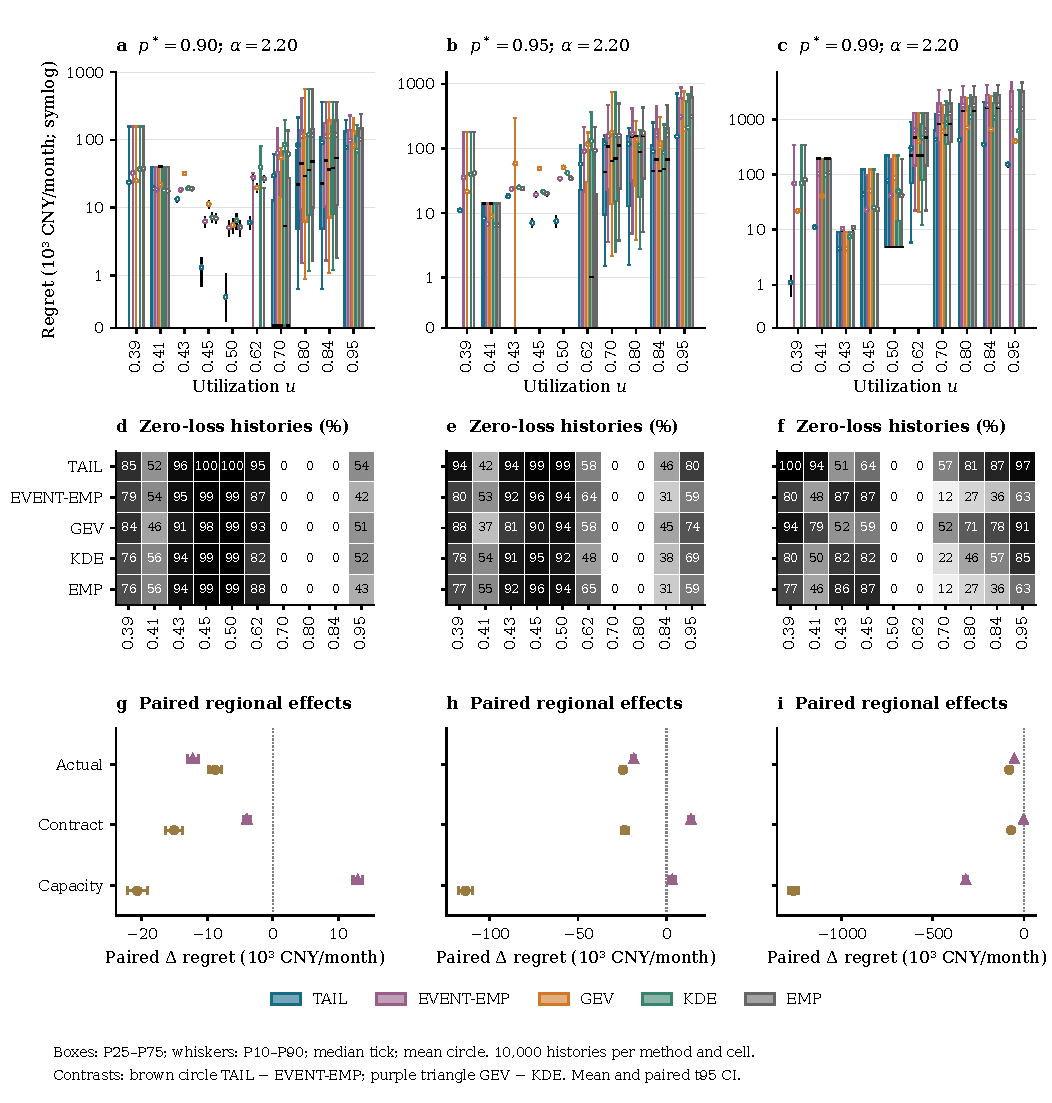
\includegraphics[width=\linewidth]{figures/FigureS1.pdf}
\caption{High-contract-quantile stress experiment at alpha = 2.20, comprising 10,000 histories, five methods, three target quantiles, and ten utilization cells per target quantile (1,500,000 decisions). Columns correspond to target quantiles 0.90, 0.95, and 0.99. (a--c) Cellwise regret distributions: boxes span P25--P75, whiskers P10--P90, black ticks denote medians, and open circles denote means; black intervals at means are pointwise 95\% Student t intervals (9,999 degrees of freedom). The symlog ordinate retains zero, is linear below one thousand CNY per month, and logarithmic above it; ranges vary by column. (d--f) Percentages of exactly zero regret, with the same grayscale mapping from 0 to 100 in all panels. Printed values are rounded to whole percentages; a printed 100 need not imply every history has zero regret. (g--i) Same-information paired regional mean differences: TAIL minus EVENT-EMP (circles) and GEV minus KDE (triangles). Cells are equally weighted within history and oracle region before differences are formed; intervals are paired t95 intervals. Negative values favour the first method. Data were reconstructed from saved fits without refitting or new simulation.}
\label{fig:final-figures1}
\end{figure}

\begin{figure}[tbp]
\centering
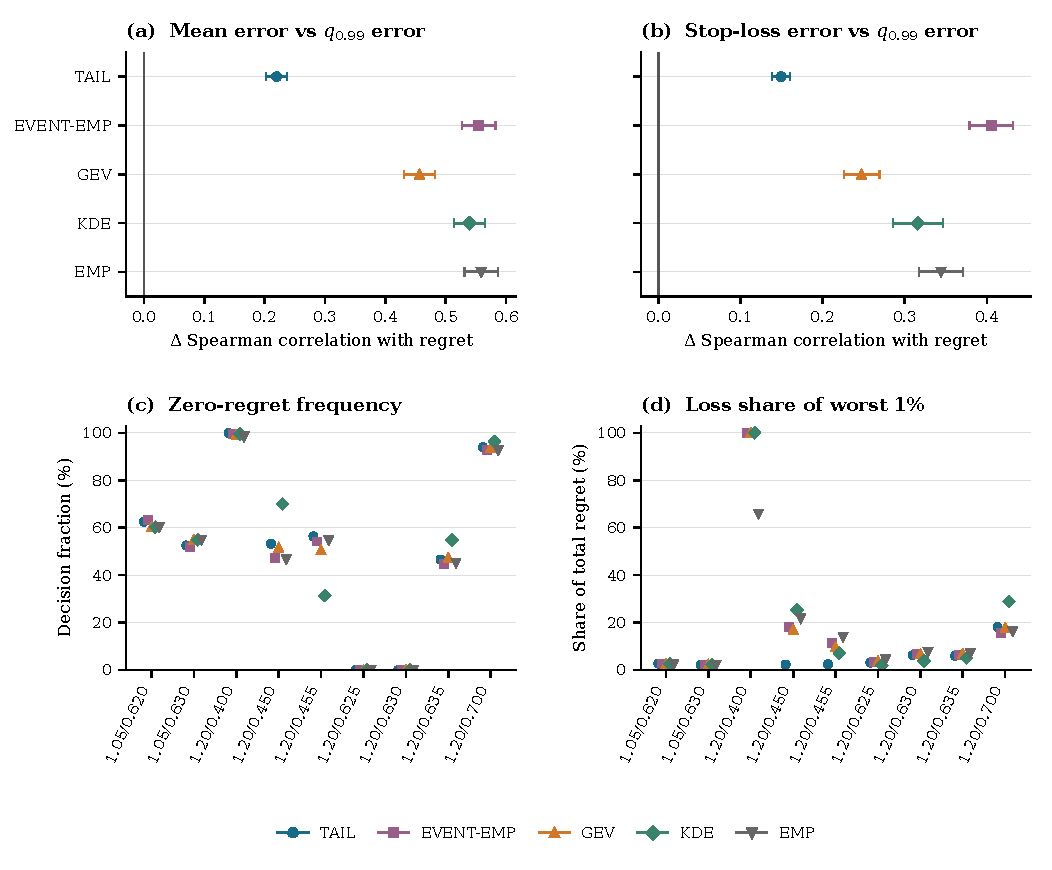
\includegraphics[width=\linewidth]{figures/FigureS2.pdf}
\caption{Functional-error associations and loss concentration. (a,b) Within-method differences between the Spearman correlation of regret with absolute mean or stop-loss relative error and its correlation with absolute $q_{0.99}$ relative error. Error and regret quantities are first averaged over nine cells within each of 10,000 histories. Intervals are the supplied simultaneous max-$|T|$ 95\% intervals for the family of ten correlation differences, based on 2,000 paired-history bootstrap resamples. They are not pointwise intervals. (c) Zero-regret frequency and (d) the share of aggregate regret accounted for by the worst 1\% of decisions within each method--cell sample. The lower panels are descriptive summaries from 10,000 histories per method and cell. Offset, unconnected points distinguish methods at discrete tariff cells; the positions do not form a continuous tariff response.}
\label{fig:final-figures2}
\end{figure}

\begin{figure}[tbp]
\centering
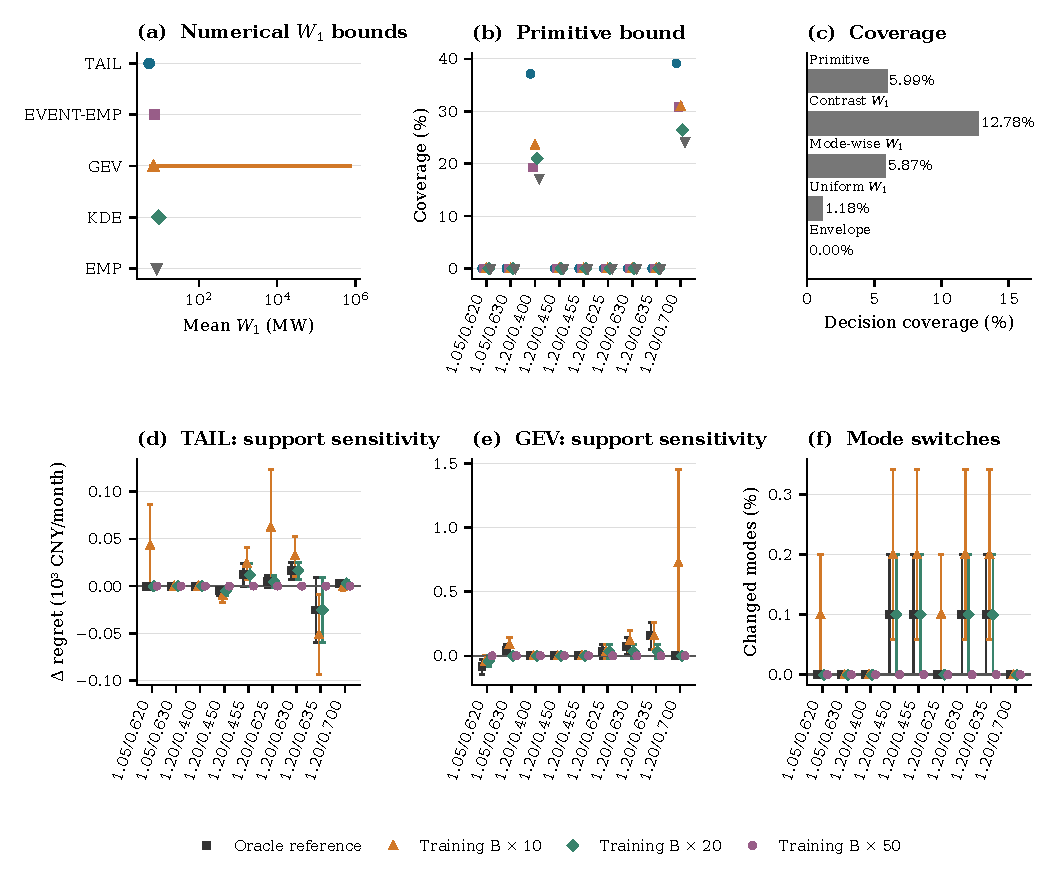
\includegraphics[width=\linewidth]{figures/FigureS3.pdf}
\caption{\textbf{Numerical distribution-to-decision bounds and
fitting-support sensitivity.}
\textbf{(a)} Mean $W_1$ point estimates and CDF-based numerical
lower and upper bounds over 10,000 fitted laws per method; the
logarithmic axis retains the loose GEV upper bound.
\textbf{(b)} Cellwise coverage of the primitive numerical
sufficient-condition check by predictive method.
\textbf{(c)} Overall coverage of the Primitive,
contrast-Wasserstein, mode-wise pairwise-Wasserstein,
uniform-Wasserstein, and coarse distributional-envelope checks over
450,000 primary decisions. The first four use the same numerical
full-action solver allowance. The contrast-Wasserstein and mode-wise
pairwise-Wasserstein checks differ in whether the common distributional
perturbation is bounded directly for each tariff contrast or after
separate mode-value bounds.
\textbf{(d,e)} Paired mean regret changes for TAIL and GEV under
alternative fitted-support rules relative to the primary
specification.
\textbf{(f)} Percentage of TAIL tariff-mode decisions that change
under each support rule. Error bars in (d--f) are one paired Monte
Carlo standard error over the first 1,000 primary histories.
Training-derived support rules use multipliers 10, 20, and 50;
Oracle reference denotes the diagnostic bound $10q_{0.999}$.
Point estimates in (a), the CDF-based bounds, and the solver
allowances are numerical rather than interval-certified quantities.}
\label{fig:final-figures3}
\end{figure}

\begin{figure}[tbp]
\centering
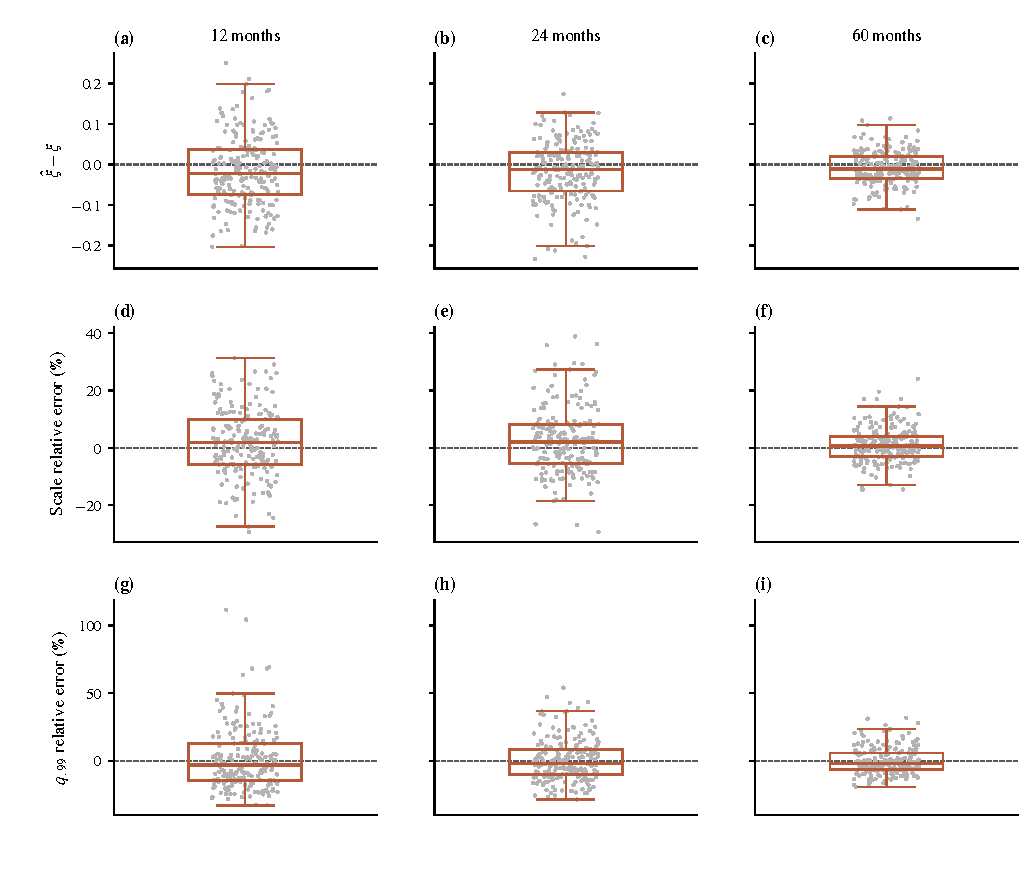
\includegraphics[width=\linewidth]{figures/FigureS4.pdf}
\caption{Parameter-recovery experiment. Columns show training
lengths of 12, 24, and 60 months; rows show GPD shape error, relative
scale error, and relative $q_{0.99}$ error. Each panel displays all
200 histories as grey points, with median, interquartile box, and
1.5-IQR whiskers. These are distribution summaries, not confidence
intervals; the recovery experiment is separate from the primary
analysis.}
\label{fig:final-figures4}
\end{figure}

\begin{figure}[tbp]
\centering
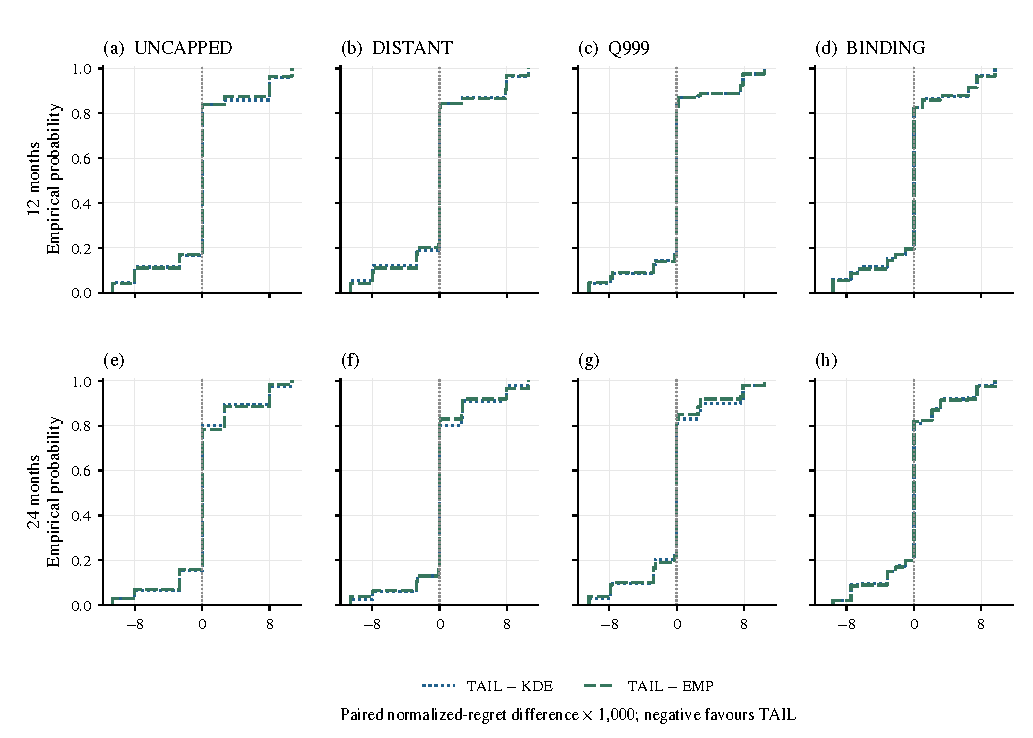
\includegraphics[width=\linewidth]{figures/FigureS5.pdf}
\caption{Physical clipping sensitivity. Columns show the four frozen
clipping regimes and rows show 12 or 24 training months. Each ECDF
contains 200 paired history differences in normalized regret times
1,000; negative values favour TAIL. The full data range is shown, and
the interquartile range is zero in all 16 groups. This descriptive
robustness experiment is separate from the primary analysis.}
\label{fig:final-figures5}
\end{figure}

\begin{figure}[tbp]
\centering
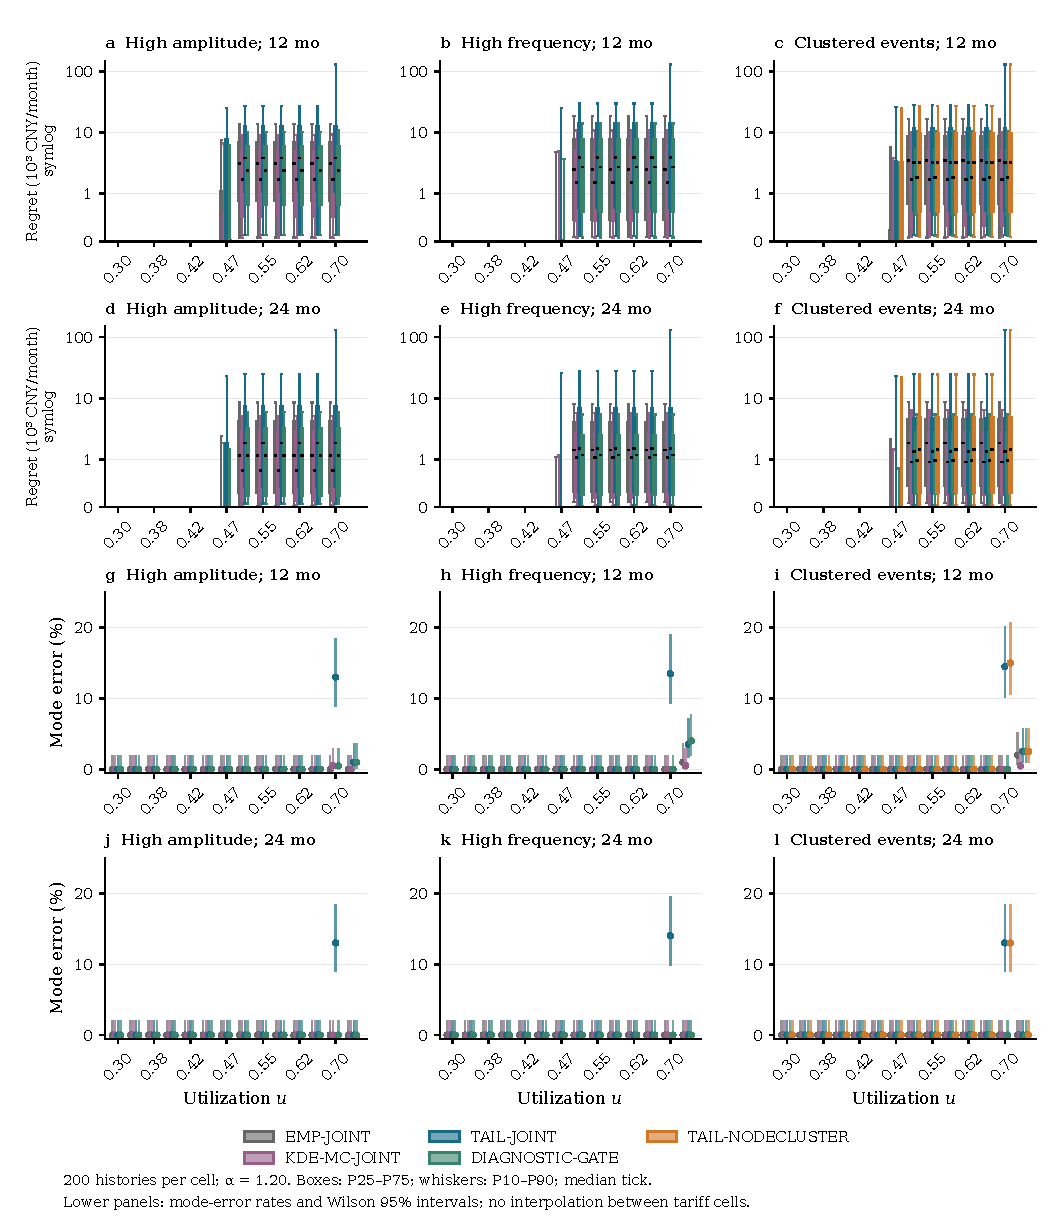
\includegraphics[width=0.94\linewidth]{figures/FigureS6.pdf}
\caption{Physical-pipeline experiments at alpha = 1.20 using 200
paired histories per method, training length, and tariff cell
(72,800 decisions). Columns represent high amplitude, high frequency,
and clustered events. (a--f) Regret distributions at all 14 utilization
cells for training lengths of 12 and 24 months: boxes span P25--P75,
whiskers span P10--P90, and black ticks denote medians. The symlog
ordinate retains zero and is linear below one thousand CNY per month.
Outlying histories beyond the whiskers are not drawn individually;
these are distribution summaries, not confidence intervals. (g--l)
Mode-error proportions and pointwise Wilson 95\% intervals at the
same cells. Points are offset within each cell to separate methods and
are not interpolated between cells. TAIL-NODECLUSTER applies only to
the clustered-event scenario.}
\label{fig:final-figures6}
\end{figure}

\begin{figure}[tbp]
\centering
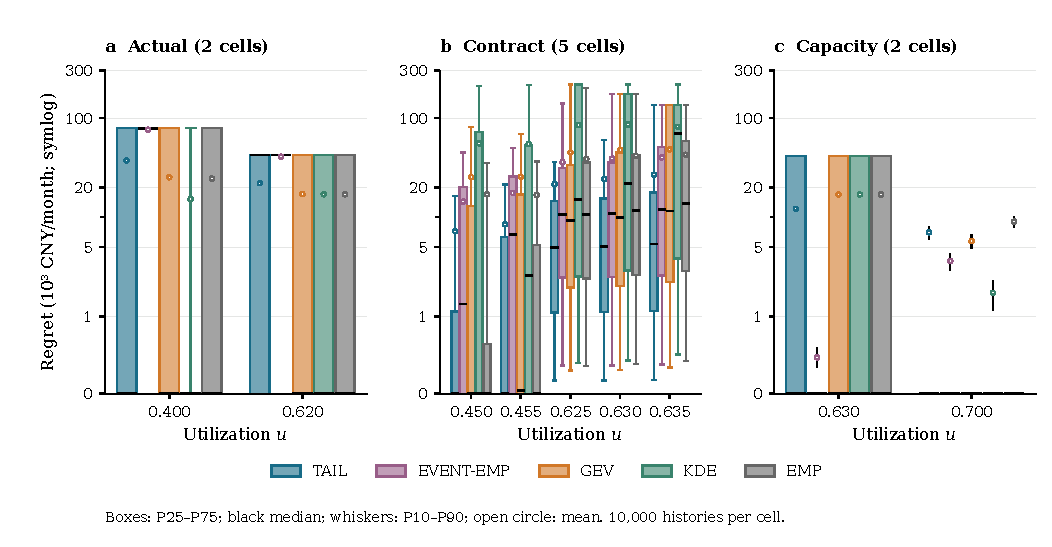
\includegraphics[width=\linewidth]{figures/FigureS7.pdf}
\caption{Cellwise regret distributions under the negative-binomial--Weibull challenge, with 10,000 histories per method and cell. Panels group the two actual, five contract, and two capacity oracle cells; labels give utilization and cells are equally spaced. Filled boxes span P25--P75, black ticks denote medians, whiskers span P10--P90, and open circles denote means. Black intervals at means use the formal pointwise normal 95\% approximation, mean plus or minus 1.96 standard errors. The symlog ordinate is linear below one thousand CNY per month and logarithmic above it. Histories outside the displayed quantile ranges are not drawn individually. Quantile ranges describe history variability and are distinct from uncertainty in the mean.}
\label{fig:final-figures7}
\end{figure}

\begin{figure}[tbp]
\centering
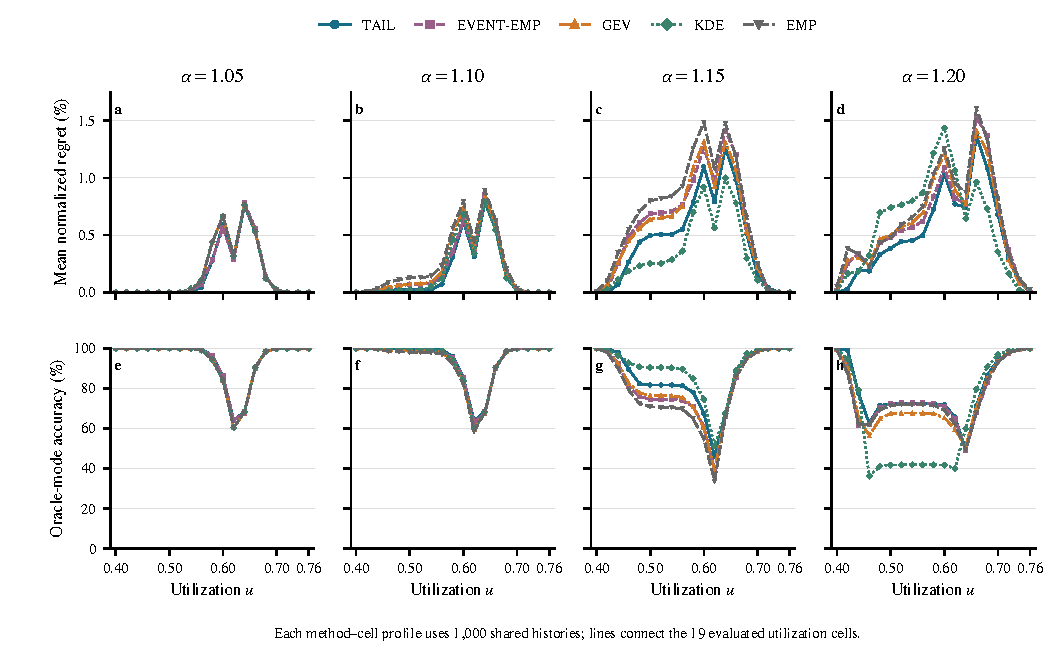
\includegraphics[width=\linewidth]{figures/FigureS8.pdf}
\caption{Complete five-method profiles over the final nonnegative, no-artificial-upper crossed tariff grid. Panels (a--d) show mean normalized full-action regret, $R/V_F^*$, and panels (e--h) show oracle-mode accuracy, for $\alpha=1.05$, 1.10, 1.15, and 1.20. Each panel covers the 19 evaluated utilization values; each method--cell estimate uses 1,000 shared histories, giving 380,000 decisions in total. Lines connect discrete evaluated cells for visual comparison and do not represent interpolation. The profiles are descriptive; no confidence intervals are shown and no invariant within-region ranking is asserted. TAIL and EVENT--EMP use event-level information; GEV, KDE, and EMP use monthly maxima.}
\label{fig:crossed-grid-all-methods}
\end{figure}



\clearpage
\subsection*{Supplementary tables}

\begingroup
\fontsize{8.5}{10.5}\selectfont\setlength{\tabcolsep}{3.0pt}\renewcommand{\arraystretch}{1.23}
\begin{table}[tbp]\centering
\caption{Same-information comparisons under high contract quantiles.}\label{tab:si-high-pstar}
\begin{tabular}{@{}llllll@{}}\toprule
$p^*$ & First -- second & Oracle & Cells & Difference & 95\% CI\\\midrule
0.90 & GEV -- KDE & Actual & 1 & -12.19 & [-13.02, -11.36]\\
0.90 & GEV -- KDE & Capacity & 1 & +12.97 & [+12.26, +13.68]\\
0.90 & GEV -- KDE & Contract & 8 & -3.97 & [-4.53, -3.41]\\
0.90 & TAIL -- EVENT-EMP & Actual & 1 & -8.80 & [-9.73, -7.87]\\
0.90 & TAIL -- EVENT-EMP & Capacity & 1 & -20.68 & [-22.18, -19.18]\\
0.90 & TAIL -- EVENT-EMP & Contract & 8 & -15.06 & [-16.39, -13.72]\\
0.95 & GEV -- KDE & Actual & 1 & -18.40 & [-19.46, -17.33]\\
0.95 & GEV -- KDE & Capacity & 2 & +3.28 & [+1.49, +5.07]\\
0.95 & GEV -- KDE & Contract & 7 & +13.97 & [+12.78, +15.15]\\
0.95 & TAIL -- EVENT-EMP & Actual & 1 & -24.59 & [-25.86, -23.31]\\
0.95 & TAIL -- EVENT-EMP & Capacity & 2 & -113.74 & [-117.77, -109.70]\\
0.95 & TAIL -- EVENT-EMP & Contract & 7 & -23.47 & [-25.59, -21.35]\\
0.99 & GEV -- KDE & Actual & 2 & -52.28 & [-54.06, -50.49]\\
0.99 & GEV -- KDE & Capacity & 4 & -318.31 & [-329.72, -306.91]\\
0.99 & GEV -- KDE & Contract & 4 & -1.37 & [-3.10, +0.36]\\
0.99 & TAIL -- EVENT-EMP & Actual & 2 & -80.28 & [-82.37, -78.19]\\
0.99 & TAIL -- EVENT-EMP & Capacity & 4 & -1261.71 & [-1288.14, -1235.28]\\
0.99 & TAIL -- EVENT-EMP & Contract & 4 & -70.45 & [-73.18, -67.71]\\
\bottomrule
\end{tabular}
\par\smallskip\noindent\begin{minipage}{\linewidth}\footnotesize Loss differences are in $10^3$ CNY/month. Each comparison uses the same 10,000 fitted primary histories and equal weights over the indicated region cells; intervals are pointwise paired $t$ intervals. Alpha is 2.20. No multiple-testing p-values are used for interpretation.\end{minipage}
\end{table}
\endgroup

\FloatBarrier

\begingroup
\fontsize{8.5}{10.5}\selectfont\setlength{\tabcolsep}{3.0pt}\renewcommand{\arraystretch}{1.23}
\begin{table}[tbp]\centering
\caption{Conditional within-contract regret by certificate status.}\label{tab:si-certificate}
\begin{tabular}{@{}lllllll@{}}\toprule
Split & Method & Certified & Decisions & Histories & Mean & 95\% CI\\\midrule
$d_{MV}$ & TAIL & Yes & 453 & 392 & 0.39 & [0.34, 0.45]\\
$d_{MV}$ & TAIL & No & 17,142 & 6,812 & 7.81 & [7.48, 8.15]\\
$d_{MV}$ & EVENT-EMP & Yes & 284 & 254 & 7.14 & [5.86, 8.43]\\
$d_{MV}$ & EVENT-EMP & No & 17,581 & 6,948 & 11.73 & [11.26, 12.20]\\
$d_{MV}$ & GEV & Yes & 228 & 208 & 4.23 & [3.50, 4.95]\\
$d_{MV}$ & GEV & No & 16,308 & 6,658 & 13.11 & [12.56, 13.65]\\
$d_{MV}$ & KDE & Yes & 144 & 131 & 12.19 & [10.42, 13.96]\\
$d_{MV}$ & KDE & No & 10,684 & 4,273 & 9.75 & [9.22, 10.28]\\
$d_{MV}$ & EMP & Yes & 221 & 201 & 8.80 & [7.11, 10.48]\\
$d_{MV}$ & EMP & No & 17,285 & 6,995 & 17.86 & [17.16, 18.56]\\
Pairwise & TAIL & Yes & 1,081 & 684 & 0.67 & [0.60, 0.73]\\
Pairwise & TAIL & No & 16,514 & 6,601 & 8.02 & [7.68, 8.36]\\
Pairwise & EVENT-EMP & Yes & 714 & 465 & 7.61 & [6.64, 8.58]\\
Pairwise & EVENT-EMP & No & 17,151 & 6,813 & 11.73 & [11.25, 12.21]\\
Pairwise & GEV & Yes & 598 & 394 & 4.42 & [3.81, 5.02]\\
Pairwise & GEV & No & 15,938 & 6,526 & 13.24 & [12.68, 13.79]\\
Pairwise & KDE & Yes & 408 & 262 & 11.93 & [10.71, 13.14]\\
Pairwise & KDE & No & 10,420 & 4,220 & 9.58 & [9.04, 10.11]\\
Pairwise & EMP & Yes & 580 & 379 & 10.04 & [8.47, 11.61]\\
Pairwise & EMP & No & 16,926 & 6,891 & 17.84 & [17.13, 18.55]\\
\bottomrule
\end{tabular}
\par\smallskip\noindent\begin{minipage}{\linewidth}\footnotesize The subset contains decisions for which both oracle and fitted-law selected modes are contract. The mean is the equally weighted mean of eligible history means, with a pointwise $t$ interval using the displayed number of histories. Loss units are $10^3$ CNY/month. Different subsets overlap across methods and certificate splits; their counts must not be added to obtain the number of independent histories.\end{minipage}
\end{table}
\endgroup

\FloatBarrier

\begingroup
\fontsize{8.5}{10.5}\selectfont\setlength{\tabcolsep}{3.0pt}\renewcommand{\arraystretch}{1.23}
\begin{table}[tbp]\centering
\caption{Physical-mechanism stress tests at alpha 1.20.}\label{tab:si-s6-updated}
\begin{tabular}{@{}llllllll@{}}\toprule
Scenario & Months & Method & Regret & MCSE & Mode & Within & Error (\%)\\\midrule
High amplitude & 12 & GATE & 2.114 & 0.236 & 0.110 & 2.005 & 0.107\\
High amplitude & 12 & EMP-JOINT & 2.512 & 0.248 & 0.000 & 2.512 & 0.000\\
High amplitude & 12 & KDE-MC-JOINT & 1.783 & 0.200 & 0.046 & 1.737 & 0.036\\
High amplitude & 12 & TAIL-JOINT & 5.740 & 0.653 & 1.267 & 4.473 & 1.000\\
High amplitude & 24 & GATE & 0.997 & 0.090 & 0.000 & 0.997 & 0.000\\
High amplitude & 24 & EMP-JOINT & 1.283 & 0.117 & 0.000 & 1.283 & 0.000\\
High amplitude & 24 & KDE-MC-JOINT & 0.842 & 0.079 & 0.000 & 0.842 & 0.000\\
High amplitude & 24 & TAIL-JOINT & 4.451 & 0.534 & 1.204 & 3.247 & 0.929\\
High frequency & 12 & GATE & 2.589 & 0.277 & 0.253 & 2.336 & 0.286\\
High frequency & 12 & EMP-JOINT & 2.731 & 0.274 & 0.063 & 2.668 & 0.071\\
High frequency & 12 & KDE-MC-JOINT & 1.784 & 0.185 & 0.032 & 1.752 & 0.036\\
High frequency & 12 & TAIL-JOINT & 5.937 & 0.621 & 1.472 & 4.464 & 1.214\\
High frequency & 24 & GATE & 0.947 & 0.090 & 0.000 & 0.947 & 0.000\\
High frequency & 24 & EMP-JOINT & 1.286 & 0.116 & 0.000 & 1.286 & 0.000\\
High frequency & 24 & KDE-MC-JOINT & 0.948 & 0.095 & 0.000 & 0.948 & 0.000\\
High frequency & 24 & TAIL-JOINT & 4.311 & 0.544 & 1.297 & 3.014 & 1.000\\
Clustered events & 12 & GATE & 2.151 & 0.264 & 0.158 & 1.993 & 0.179\\
Clustered events & 12 & EMP-JOINT & 3.135 & 0.315 & 0.127 & 3.009 & 0.143\\
Clustered events & 12 & KDE-MC-JOINT & 1.855 & 0.217 & 0.032 & 1.823 & 0.036\\
Clustered events & 12 & TAIL-JOINT & 5.303 & 0.582 & 1.502 & 3.801 & 1.214\\
Clustered events & 12 & TAIL-NODECLUSTER & 5.380 & 0.595 & 1.548 & 3.832 & 1.250\\
Clustered events & 24 & GATE & 0.936 & 0.093 & 0.000 & 0.936 & 0.000\\
Clustered events & 24 & EMP-JOINT & 1.572 & 0.145 & 0.000 & 1.572 & 0.000\\
Clustered events & 24 & KDE-MC-JOINT & 1.020 & 0.105 & 0.000 & 1.020 & 0.000\\
Clustered events & 24 & TAIL-JOINT & 3.782 & 0.513 & 1.205 & 2.577 & 0.929\\
Clustered events & 24 & TAIL-NODECLUSTER & 3.768 & 0.510 & 1.205 & 2.563 & 0.929\\
\bottomrule
\end{tabular}
\par\smallskip\noindent\begin{minipage}{\linewidth}\footnotesize Each scenario-by-training-length summary uses 200 independent histories, each evaluated at 14 equally weighted tariff cells (2,800 decision rows). GATE denotes DIAGNOSTIC-GATE. Losses are in $10^3$ CNY/month. MCSE is calculated after averaging cells within history. The oracle is a fixed independent synthetic test pool.\end{minipage}
\end{table}
\endgroup

\FloatBarrier

\begingroup
\fontsize{8.5}{10.5}\selectfont\setlength{\tabcolsep}{3pt}
\begin{longtable}{@{}llllll@{}}
\caption{Cell-specific NB--Weibull challenge results.}\label{tab:final-si-4}\\
\toprule
Region & Alpha / u & Method & Mean regret & 95\% CI & Accuracy (\%)\\\midrule\endfirsthead
Region & Alpha / u & Method & Mean regret & 95\% CI & Accuracy (\%)\\\midrule\endhead
actual & 1.05 / 0.620 & EMP & 17.05 & [16.64, 17.45] & 59.7\\
capacity & 1.05 / 0.630 & EMP & 16.96 & [16.56, 17.36] & 59.3\\
actual & 1.20 / 0.400 & EMP & 24.55 & [23.83, 25.27] & 68.9\\
contract & 1.20 / 0.450 & EMP & 17.01 & [16.01, 18.01] & 93.9\\
capacity & 1.20 / 0.700 & EMP & 9.05 & [7.83, 10.27] & 97.9\\
contract & 1.20 / 0.635 & EMP & 42.65 & [41.53, 43.77] & 81.3\\
contract & 1.20 / 0.625 & EMP & 38.49 & [37.23, 39.76] & 90.1\\
contract & 1.20 / 0.630 & EMP & 41.54 & [40.31, 42.77] & 86.2\\
contract & 1.20 / 0.455 & EMP & 16.82 & [15.86, 17.79] & 94.8\\
actual & 1.05 / 0.620 & EVENT-EMP & 40.83 & [40.64, 41.02] & 3.7\\
capacity & 1.05 / 0.630 & EVENT-EMP & 0.47 & [0.34, 0.60] & 99.0\\
actual & 1.20 / 0.400 & EVENT-EMP & 76.46 & [76.18, 76.73] & 3.2\\
contract & 1.20 / 0.450 & EVENT-EMP & 14.39 & [13.91, 14.87] & 100.0\\
capacity & 1.20 / 0.700 & EVENT-EMP & 3.62 & [2.90, 4.34] & 99.0\\
contract & 1.20 / 0.635 & EVENT-EMP & 40.05 & [39.01, 41.09] & 77.4\\
contract & 1.20 / 0.625 & EVENT-EMP & 35.85 & [34.61, 37.08] & 90.0\\
contract & 1.20 / 0.630 & EVENT-EMP & 39.05 & [37.86, 40.24] & 84.5\\
contract & 1.20 / 0.455 & EVENT-EMP & 17.60 & [17.09, 18.10] & 100.0\\
actual & 1.05 / 0.620 & GEV & 17.11 & [16.70, 17.52] & 59.6\\
capacity & 1.05 / 0.630 & GEV & 16.89 & [16.49, 17.29] & 59.4\\
actual & 1.20 / 0.400 & GEV & 25.29 & [24.56, 26.01] & 68.0\\
contract & 1.20 / 0.450 & GEV & 25.41 & [24.24, 26.59] & 91.2\\
capacity & 1.20 / 0.700 & GEV & 5.75 & [4.79, 6.71] & 98.6\\
contract & 1.20 / 0.635 & GEV & 48.33 & [47.07, 49.58] & 73.5\\
contract & 1.20 / 0.625 & GEV & 44.86 & [43.38, 46.34] & 84.6\\
contract & 1.20 / 0.630 & GEV & 47.69 & [46.29, 49.10] & 79.8\\
contract & 1.20 / 0.455 & GEV & 25.59 & [24.45, 26.74] & 92.2\\
actual & 1.05 / 0.620 & KDE & 17.05 & [16.64, 17.45] & 59.7\\
capacity & 1.05 / 0.630 & KDE & 16.96 & [16.56, 17.36] & 59.3\\
actual & 1.20 / 0.400 & KDE & 15.23 & [14.62, 15.84] & 80.7\\
contract & 1.20 / 0.450 & KDE & 55.44 & [53.71, 57.17] & 75.9\\
capacity & 1.20 / 0.700 & KDE & 1.73 & [1.16, 2.30] & 99.6\\
contract & 1.20 / 0.635 & KDE & 81.62 & [80.10, 83.14] & 50.8\\
contract & 1.20 / 0.625 & KDE & 85.43 & [83.46, 87.40] & 63.7\\
contract & 1.20 / 0.630 & KDE & 86.07 & [84.29, 87.84] & 57.7\\
contract & 1.20 / 0.455 & KDE & 54.95 & [53.22, 56.67] & 77.5\\
actual & 1.05 / 0.620 & TAIL & 22.02 & [21.61, 22.44] & 47.9\\
capacity & 1.05 / 0.630 & TAIL & 12.15 & [11.78, 12.52] & 70.8\\
actual & 1.20 / 0.400 & TAIL & 37.34 & [36.56, 38.11] & 52.8\\
contract & 1.20 / 0.450 & TAIL & 7.21 & [6.66, 7.76] & 98.3\\
capacity & 1.20 / 0.700 & TAIL & 7.04 & [5.99, 8.09] & 98.3\\
contract & 1.20 / 0.635 & TAIL & 26.88 & [25.93, 27.83] & 85.8\\
contract & 1.20 / 0.625 & TAIL & 21.53 & [20.53, 22.53] & 94.1\\
contract & 1.20 / 0.630 & TAIL & 24.26 & [23.26, 25.26] & 90.9\\
contract & 1.20 / 0.455 & TAIL & 8.49 & [7.96, 9.03] & 98.6\\
\bottomrule
\end{longtable}
\noindent\footnotesize 10,000 histories per method and cell. Losses are in $10^3$ CNY/month; intervals use mean $\pm1.96$ SE. The oracle design has two actual, five contract and two capacity cells.
\endgroup

\FloatBarrier

\begingroup
\fontsize{8.5}{10.5}\selectfont\setlength{\tabcolsep}{3pt}
\begin{longtable}{@{}llll@{}}
\caption{Complete regional paired NB--Weibull contrasts.}\label{tab:final-si-5}\\
\toprule
Region & First -- second & Mean difference & 95\% CI\\\midrule\endfirsthead
Region & First -- second & Mean difference & 95\% CI\\\midrule\endhead
actual & TAIL -- EVENT-EMP & -28.97 & [-29.53, -28.40]\\
actual & TAIL -- GEV & +8.48 & [+7.98, +8.99]\\
actual & TAIL -- KDE & +13.54 & [+13.04, +14.05]\\
actual & TAIL -- EMP & +8.88 & [+8.37, +9.39]\\
actual & EVENT-EMP -- GEV & +37.45 & [+36.91, +37.99]\\
actual & EVENT-EMP -- KDE & +42.51 & [+42.03, +42.98]\\
actual & EVENT-EMP -- EMP & +37.85 & [+37.31, +38.38]\\
actual & GEV -- KDE & +5.06 & [+4.80, +5.32]\\
actual & GEV -- EMP & +0.40 & [+0.25, +0.55]\\
actual & KDE -- EMP & -4.66 & [-4.91, -4.41]\\
capacity & TAIL -- EVENT-EMP & +7.55 & [+7.10, +8.00]\\
capacity & TAIL -- GEV & -1.73 & [-2.19, -1.27]\\
capacity & TAIL -- KDE & +0.25 & [-0.28, +0.78]\\
capacity & TAIL -- EMP & -3.41 & [-3.91, -2.91]\\
capacity & EVENT-EMP -- GEV & -9.28 & [-9.70, -8.86]\\
capacity & EVENT-EMP -- KDE & -7.30 & [-7.74, -6.87]\\
capacity & EVENT-EMP -- EMP & -10.96 & [-11.49, -10.44]\\
capacity & GEV -- KDE & +1.98 & [+1.58, +2.37]\\
capacity & GEV -- EMP & -1.68 & [-2.04, -1.33]\\
capacity & KDE -- EMP & -3.66 & [-4.20, -3.12]\\
contract & TAIL -- EVENT-EMP & -11.71 & [-12.37, -11.05]\\
contract & TAIL -- GEV & -20.70 & [-21.69, -19.71]\\
contract & TAIL -- KDE & -55.02 & [-56.50, -53.55]\\
contract & TAIL -- EMP & -13.63 & [-14.49, -12.76]\\
contract & EVENT-EMP -- GEV & -8.99 & [-9.99, -7.99]\\
contract & EVENT-EMP -- KDE & -43.31 & [-44.77, -41.86]\\
contract & EVENT-EMP -- EMP & -1.91 & [-2.83, -1.00]\\
contract & GEV -- KDE & -34.32 & [-35.51, -33.14]\\
contract & GEV -- EMP & +7.08 & [+6.46, +7.69]\\
contract & KDE -- EMP & +41.40 & [+40.08, +42.71]\\
\bottomrule
\end{longtable}
\noindent\footnotesize Within each history, cells in the oracle region are equally weighted. There are 10,000 paired history differences per contrast. Units: $10^3$ CNY/month; intervals: mean $\pm1.96$ paired SE. Negative differences mean lower regret for the first method.
\endgroup

\FloatBarrier

\begingroup
\fontsize{8.5}{10.5}\selectfont\setlength{\tabcolsep}{3pt}
\begin{longtable}{@{}llll@{}}
\caption{Numerical Wasserstein brackets.}\label{tab:final-si-6}\\
\toprule
Method & Mean W1 (MW) & Mean lower (MW) & Mean upper (MW)\\\midrule\endfirsthead
Method & Mean W1 (MW) & Mean lower (MW) & Mean upper (MW)\\\midrule\endhead
EMP & 8.39 & 8.14 & 8.63\\
EVENT-EMP & 7.34 & 7.12 & 7.55\\
GEV & 6.99 & 5.76 & 7.33e+05\\
KDE & 9.43 & 8.92 & 9.94\\
TAIL & 5.35 & 4.68 & 6.14\\
\bottomrule
\end{longtable}
\noindent\footnotesize The $W_1$ point estimates are 256-point Gauss--Legendre numerical quadrature estimates. The CDF-based lower and upper columns are numerical bounds, not sampling confidence intervals or interval-certified enclosures. For GEV, the point estimate and CDF calculations use the fitted law conditioned on its nonnegative natural support.
\endgroup

\FloatBarrier

\begingroup
\fontsize{8.5}{10.5}\selectfont\setlength{\tabcolsep}{3pt}
\begin{longtable}{@{}llll@{}}
\caption{Functional-error correlation contrasts.}\label{tab:final-si-7}\\
\toprule
Method & Contrast & Estimate & Simultaneous 95\% CI\\\midrule\endfirsthead
Method & Contrast & Estimate & Simultaneous 95\% CI\\\midrule\endhead
TAIL & Mean -- q99 & +0.220 & [+0.203, +0.237]\\
TAIL & Stop-loss -- q99 & +0.149 & [+0.139, +0.160]\\
EVENT-EMP & Mean -- q99 & +0.555 & [+0.527, +0.583]\\
EVENT-EMP & Stop-loss -- q99 & +0.405 & [+0.379, +0.432]\\
GEV & Mean -- q99 & +0.457 & [+0.430, +0.483]\\
GEV & Stop-loss -- q99 & +0.247 & [+0.226, +0.269]\\
KDE & Mean -- q99 & +0.539 & [+0.514, +0.565]\\
KDE & Stop-loss -- q99 & +0.316 & [+0.285, +0.347]\\
EMP & Mean -- q99 & +0.559 & [+0.531, +0.587]\\
EMP & Stop-loss -- q99 & +0.344 & [+0.317, +0.371]\\
\bottomrule
\end{longtable}
\noindent\footnotesize The supplied max-$|T|$ intervals cover the family of ten within-method correlation differences. Resampling unit: history; 2,000 paired bootstrap resamples. Nine cells are averaged within each of 10,000 histories.
\endgroup

\FloatBarrier

\begingroup
\fontsize{8.5}{10.5}\selectfont\setlength{\tabcolsep}{3pt}
\begin{longtable}{@{}lll@{}}
\caption{External fit-status counts, natural-tail variant.}\label{tab:final-si-8}\\
\toprule
Method & Formal fit status & Factory-origin fits\\\midrule\endfirsthead
Method & Formal fit status & Factory-origin fits\\\midrule\endhead
K-BLOCK & PASS & 32\\
K-EMP & PASS & 32\\
K-GEV & FALLBACK\_EMPIRICAL & 24\\
K-GEV & PASS & 8\\
K-GTAIL & FALLBACK\_EMPIRICAL & 4\\
K-GTAIL & FALLBACK\_EXPONENTIAL & 13\\
K-GTAIL & PASS & 15\\
K-KDE & PASS & 32\\
K-POINT & PASS & 32\\
K-UGPD & PASS & 32\\
\bottomrule
\end{longtable}
\noindent\footnotesize Eight factories and four rolling origins yield 32 fits per method. Labels are the formal stored status labels; fallback fits remain part of the evaluated pipeline.
\endgroup

\FloatBarrier

\begingroup
\fontsize{8.5}{10.5}\selectfont\setlength{\tabcolsep}{3pt}
\begin{longtable}{@{}llll@{}}
\caption{External predictive-score paired contrasts.}\label{tab:final-si-9}\\
\toprule
Score & Baseline & GTAIL -- baseline & 95\% CI\\\midrule\endfirsthead
Score & Baseline & GTAIL -- baseline & 95\% CI\\\midrule\endhead
crps & K-BLOCK & +5.627 & [-9.534, +20.789]\\
crps & K-EMP & +3.005 & [-13.858, +19.869]\\
crps & K-GEV & +3.002 & [-14.318, +20.323]\\
crps & K-KDE & +4.654 & [-11.430, +20.737]\\
qwcrps\_090 & K-BLOCK & -0.510 & [-1.895, +0.876]\\
qwcrps\_090 & K-EMP & -0.510 & [-1.895, +0.876]\\
qwcrps\_090 & K-GEV & -0.613 & [-2.177, +0.950]\\
qwcrps\_090 & K-KDE & -0.087 & [-0.938, +0.765]\\
q95\_pinball & K-BLOCK & -2.594 & [-10.152, +4.964]\\
q95\_pinball & K-EMP & -2.594 & [-10.152, +4.964]\\
q95\_pinball & K-GEV & -3.268 & [-11.774, +5.239]\\
q95\_pinball & K-KDE & -0.548 & [-5.256, +4.161]\\
q99\_pinball & K-BLOCK & -4.071 & [-11.427, +3.285]\\
q99\_pinball & K-EMP & -4.071 & [-11.427, +3.285]\\
q99\_pinball & K-GEV & -4.481 & [-12.648, +3.687]\\
q99\_pinball & K-KDE & -0.050 & [-2.356, +2.256]\\
\bottomrule
\end{longtable}
\noindent\footnotesize Scores and intervals are multiplied by $10^3$. Each factory averages four origins; pointwise paired $t$ intervals use eight factory differences and seven degrees of freedom. Score-specific comparisons are descriptive.
\endgroup

\FloatBarrier

% Requires booktabs, array, longtable.
{\small
\begin{longtable}{>{\raggedright\arraybackslash}p{68.49pt}>{\raggedright\arraybackslash}p{91.31pt}>{\raggedright\arraybackslash}p{114.14pt}>{\raggedright\arraybackslash}p{182.63pt}}
\caption{Conditional parameter-interval coverage}\label{tab:table_s10}\\
\toprule
\textbf{Months} & \textbf{Parameter} & \textbf{Covered /\allowbreak{} histories} & \textbf{Coverage (\%) [95\% MC CI]} \\
\midrule\endfirsthead
\toprule
\textbf{Months} & \textbf{Parameter} & \textbf{Covered /\allowbreak{} histories} & \textbf{Coverage (\%) [95\% MC CI]} \\
\midrule\endhead
\bottomrule\endfoot
12 & xi & 182 /\allowbreak{} 200 & 91.00 [86.15, 94.58] \\
12 & sigma & 190 /\allowbreak{} 200 & 95.00 [91.00, 97.58] \\
24 & xi & 185 /\allowbreak{} 200 & 92.50 [87.93, 95.74] \\
24 & sigma & 182 /\allowbreak{} 200 & 91.00 [86.15, 94.58] \\
60 & xi & 190 /\allowbreak{} 200 & 95.00 [91.00, 97.58] \\
60 & sigma & 191 /\allowbreak{} 200 & 95.50 [91.63, 97.92] \\
\end{longtable}
\noindent{\footnotesize Separate inherited recovery experiment, 200 histories per setting; not the primary experiment. Coverage conditions on the selected threshold. Clopper--Pearson intervals describe Monte Carlo uncertainty in coverage.\par}
}

\FloatBarrier

\begingroup
\fontsize{8.5}{10.5}\selectfont\setlength{\tabcolsep}{3pt}
\begin{longtable}{@{}llllllll@{}}
\caption{Fitting-support policy sensitivity.}\label{tab:final-si-11}\\
\toprule
Alpha / u & Policy & TAIL delta R & SE & Mode (\%) & GEV delta R & SE & Mode (\%)\\\midrule\endfirsthead
Alpha / u & Policy & TAIL delta R & SE & Mode (\%) & GEV delta R & SE & Mode (\%)\\\midrule\endhead
1.05/0.620 & Oracle reference & +0.000 & 0.000 & 0.00 & -0.086 & 0.061 & 0.20\\
1.05/0.630 & Oracle reference & +0.000 & 0.000 & 0.00 & +0.042 & 0.042 & 0.10\\
1.20/0.400 & Oracle reference & +0.000 & 0.000 & 0.00 & +0.000 & 0.000 & 0.00\\
1.20/0.450 & Oracle reference & -0.005 & 0.005 & 0.10 & -0.000 & 0.000 & 0.00\\
1.20/0.700 & Oracle reference & +0.003 & 0.003 & 0.00 & +0.000 & 0.000 & 0.00\\
1.20/0.635 & Oracle reference & -0.025 & 0.034 & 0.10 & +0.155 & 0.107 & 0.40\\
1.20/0.625 & Oracle reference & +0.004 & 0.006 & 0.00 & +0.032 & 0.053 & 0.20\\
1.20/0.630 & Oracle reference & +0.016 & 0.009 & 0.10 & +0.074 & 0.068 & 0.30\\
1.20/0.455 & Oracle reference & +0.012 & 0.012 & 0.10 & -0.000 & 0.000 & 0.00\\
1.05/0.620 & Training x10 & +0.043 & 0.043 & 0.10 & -0.043 & 0.043 & 0.10\\
1.05/0.630 & Training x10 & +0.000 & 0.000 & 0.00 & +0.085 & 0.060 & 0.20\\
1.20/0.400 & Training x10 & +0.000 & 0.000 & 0.00 & +0.000 & 0.000 & 0.00\\
1.20/0.450 & Training x10 & -0.010 & 0.007 & 0.20 & -0.000 & 0.000 & 0.00\\
1.20/0.700 & Training x10 & -0.000 & 0.004 & 0.00 & +0.726 & 0.726 & 0.10\\
1.20/0.635 & Training x10 & -0.052 & 0.042 & 0.20 & +0.155 & 0.107 & 0.40\\
1.20/0.625 & Training x10 & +0.062 & 0.061 & 0.10 & +0.032 & 0.053 & 0.20\\
1.20/0.630 & Training x10 & +0.032 & 0.021 & 0.20 & +0.117 & 0.080 & 0.40\\
1.20/0.455 & Training x10 & +0.024 & 0.017 & 0.20 & -0.000 & 0.000 & 0.00\\
1.05/0.620 & Training x20 & +0.000 & 0.000 & 0.00 & -0.043 & 0.043 & 0.10\\
1.05/0.630 & Training x20 & +0.000 & 0.000 & 0.00 & +0.000 & 0.000 & 0.00\\
1.20/0.400 & Training x20 & +0.000 & 0.000 & 0.00 & +0.000 & 0.000 & 0.00\\
1.20/0.450 & Training x20 & -0.005 & 0.005 & 0.10 & -0.000 & 0.000 & 0.00\\
1.20/0.700 & Training x20 & +0.003 & 0.003 & 0.00 & +0.000 & 0.000 & 0.00\\
1.20/0.635 & Training x20 & -0.025 & 0.034 & 0.10 & +0.032 & 0.053 & 0.20\\
1.20/0.625 & Training x20 & +0.004 & 0.006 & 0.00 & +0.032 & 0.053 & 0.20\\
1.20/0.630 & Training x20 & +0.016 & 0.009 & 0.10 & +0.032 & 0.053 & 0.20\\
1.20/0.455 & Training x20 & +0.012 & 0.012 & 0.10 & -0.000 & 0.000 & 0.00\\
1.05/0.620 & Training x50 & +0.000 & 0.000 & 0.00 & +0.000 & 0.000 & 0.00\\
1.05/0.630 & Training x50 & +0.000 & 0.000 & 0.00 & +0.000 & 0.000 & 0.00\\
1.20/0.400 & Training x50 & +0.000 & 0.000 & 0.00 & +0.000 & 0.000 & 0.00\\
1.20/0.450 & Training x50 & +0.000 & 0.000 & 0.00 & -0.000 & 0.000 & 0.00\\
1.20/0.700 & Training x50 & +0.000 & 0.000 & 0.00 & +0.000 & 0.000 & 0.00\\
1.20/0.635 & Training x50 & +0.000 & 0.000 & 0.00 & +0.000 & 0.000 & 0.00\\
1.20/0.625 & Training x50 & +0.000 & 0.000 & 0.00 & +0.000 & 0.000 & 0.00\\
1.20/0.630 & Training x50 & +0.000 & 0.000 & 0.00 & +0.000 & 0.000 & 0.00\\
1.20/0.455 & Training x50 & +0.000 & 0.000 & 0.00 & -0.000 & 0.000 & 0.00\\
\bottomrule
\end{longtable}
\noindent\footnotesize The TAIL and GEV column blocks each give paired mean change in regret, paired SE, and changed-mode percentage. All differences are relative to the primary support specification. The first 1,000 paired histories form this separate support audit. Loss and SE units: $10^3$ CNY/month. This subset does not replace the 10,000-history primary experiment.
\endgroup

\FloatBarrier

\begingroup
\fontsize{8.5}{10.5}\selectfont\setlength{\tabcolsep}{3.0pt}\renewcommand{\arraystretch}{1.23}
\begin{table}[tbp]\centering
\caption{Complete history-paired regret contrasts in the primary experiment.}\label{tab:final-si-12}
\begin{tabular}{@{}llll@{}}\toprule
First -- second & Actual & Contract & Capacity\\\midrule
TAIL -- EVENT-EMP & \shortstack{-0.61\\{}[-0.77, -0.44]} & \shortstack{-1.68\\{}[-1.93, -1.43]} & \shortstack{-2.67\\{}[-3.24, -2.10]}\\
GEV -- KDE & \shortstack{+0.82\\{}[+0.68, +0.97]} & \shortstack{-3.89\\{}[-4.14, -3.63]} & \shortstack{+5.47\\{}[+4.87, +6.07]}\\
KDE -- EMP & \shortstack{-1.66\\{}[-1.88, -1.43]} & \shortstack{+1.73\\{}[+1.40, +2.06]} & \shortstack{-8.71\\{}[-9.41, -8.00]}\\
TAIL -- KDE & \shortstack{-0.66\\{}[-0.85, -0.47]} & \shortstack{-7.38\\{}[-7.69, -7.06]} & \shortstack{+4.13\\{}[+3.44, +4.81]}\\
TAIL -- GEV & \shortstack{-1.48\\{}[-1.72, -1.24]} & \shortstack{-3.49\\{}[-3.77, -3.22]} & \shortstack{-1.34\\{}[-1.98, -0.70]}\\
TAIL -- EMP & \shortstack{-2.32\\{}[-2.62, -2.01]} & \shortstack{-5.65\\{}[-5.99, -5.31]} & \shortstack{-4.58\\{}[-5.26, -3.89]}\\
GEV -- EMP & \shortstack{-0.84\\{}[-1.01, -0.66]} & \shortstack{-2.16\\{}[-2.37, -1.95]} & \shortstack{-3.23\\{}[-3.62, -2.85]}\\
EVENT-EMP -- GEV & \shortstack{-0.88\\{}[-1.12, -0.63]} & \shortstack{-1.81\\{}[-2.05, -1.57]} & \shortstack{+1.33\\{}[+0.77, +1.89]}\\
EVENT-EMP -- KDE & \shortstack{-0.05\\{}[-0.26, +0.15]} & \shortstack{-5.70\\{}[-5.99, -5.40]} & \shortstack{+6.80\\{}[+6.10, +7.50]}\\
EVENT-EMP -- EMP & \shortstack{-1.71\\{}[-1.99, -1.43]} & \shortstack{-3.97\\{}[-4.25, -3.68]} & \shortstack{-1.90\\{}[-2.46, -1.35]}\\
\bottomrule
\end{tabular}
\par\smallskip\noindent\begin{minipage}{\linewidth}\footnotesize First method minus second, in $10^3$ CNY/month; negative values favour the first method. Brackets are pointwise paired $t$ 95\% intervals from 10,000 equally weighted regional history means (9,999 degrees of freedom). The first two comparisons share event histories and monthly maxima, respectively; the remaining comparisons provide descriptive context. Intervals are not simultaneous and are not interpreted as family-wise evidence.\end{minipage}
\end{table}
\endgroup

\FloatBarrier

\begingroup
\small
\setlength{\tabcolsep}{2.5pt}
\renewcommand{\arraystretch}{1.12}
\begin{table}[tbp]
\centering
\caption{Primary tariff geometry and analytic demand-scale stability radii.}
\label{tab:analytic-demand-radii}
\resizebox{\linewidth}{!}{%
\begin{tabular}{@{}rrlrrrrrr@{}}
\toprule
$\alpha$ & Utilization & Oracle mode & $V_F^*$ & $\gamma_F$ & Relative gap & $\rho_F^{\mathrm{contrast}}$ & $\rho_F^{\mathrm{pair}}$ & $\rho_F$ \\
& & & \shortstack{($10^3$ CNY/month)} & \shortstack{($10^3$ CNY/month)} & (\%) & (kW) & (kW) & (kW) \\
\midrule
1.05 & 0.620 & Actual & 5,336.473 & 43.036 & 0.806 & 1,195.45 & 1,195.45 & 298.86 \\
1.05 & 0.630 & Capacity & 5,294.120 & 42.353 & 0.800 & 1,176.47 & 1,176.47 & 294.12 \\
1.20 & 0.400 & Actual & 5,336.473 & 318.649 & 5.971 & 8,851.37 & 2,950.46 & 2,212.84 \\
1.20 & 0.450 & Actual & 5,336.473 & 4.962 & 0.093 & 137.84 & 45.95 & 34.46 \\
1.20 & 0.455 & Contract & 5,324.612 & 11.861 & 0.223 & 329.48 & 109.83 & 82.37 \\
1.20 & 0.625 & Contract & 5,276.065 & 60.408 & 1.145 & 839.00 & 559.34 & 419.50 \\
1.20 & 0.630 & Contract & 5,276.065 & 18.055 & 0.342 & 250.77 & 250.77 & 125.38 \\
1.20 & 0.635 & Capacity & 5,252.434 & 23.631 & 0.450 & 328.20 & 328.20 & 164.10 \\
1.20 & 0.700 & Capacity & 4,764.708 & 511.357 & 10.732 & 7,102.18 & 7,102.18 & 3,551.09 \\
\bottomrule
\end{tabular}}
\par\smallskip
\begin{minipage}{\linewidth}\footnotesize $V_F^*$ and $\gamma_F$ are in thousand CNY/month; relative gap is $100\gamma_F/V_F^*$. The direct contrast radius is $\rho_F^{\mathrm{contrast}}=\min_{m\neq m_F^*}\gamma_{F,m}/K_{m,m_F^*}$; the mode-wise pairwise radius is $\rho_F^{\mathrm{pair}}=\min_{m\neq m_F^*}\gamma_{F,m}/(L_m+L_{m_F^*})$; and the uniform radius is $\rho_F=\gamma_F/(2L)$ with $L=r_d\max\{1,\kappa\}$. All are oracle-dependent analytic quantities in kW and contain no numerical-integration or solver allowance. For the primary coefficients, $\kappa=2$, so $K_{\mathrm{act},\mathrm{con}}=36$ CNY/kW compared with $L_{\mathrm{act}}+L_{\mathrm{con}}=108$ CNY/kW. Across these cells, $\rho_F^{\mathrm{contrast}}\geq\rho_F^{\mathrm{pair}}\geq\rho_F$.\end{minipage}
\end{table}
\endgroup

\FloatBarrier

\begingroup
\small
\setlength{\tabcolsep}{5pt}
\renewcommand{\arraystretch}{1.15}
\begin{table}[tbp]
\centering
\caption{Numerical sufficient-condition implementation audit.}
\label{tab:numerical-sufficient-condition-audit}
\begin{tabular}{@{}lrrr@{}}
\toprule
Condition & Passing rows & Coverage (\%) & Observed mode-selection violations \\
\midrule
Primitive numerical check & 26,975 & 5.994444 & 0 \\
Contrast-Wasserstein numerical check & 57,501 & 12.778000 & 0 \\
Mode-wise pairwise-Wasserstein numerical check & 26,393 & 5.865111 & 0 \\
Uniform-Wasserstein numerical check & 5,329 & 1.184222 & 0 \\
\bottomrule
\end{tabular}
\par\smallskip
\begin{minipage}{\linewidth}\footnotesize The primitive check is $2\varepsilon_{\rm num}+\zeta_{\rm full,num}<\gamma_F$. The contrast-Wasserstein check requires $K_{m,m_F^*}W_{1,\rm upper}+\zeta_{\rm full,num}<\gamma_{F,m}$ for every competing mode, using the direct tariff-contrast constants defined in Section S1.7. The mode-wise pairwise check replaces $K_{m,m_F^*}$ by $L_m+L_{m_F^*}$; the uniform check is $2LW_{1,\rm upper}+\zeta_{\rm full,num}<\gamma_F$, where $L=r_d\max\{1,\kappa\}$. All four use the same numerical full-action solver allowance. No observed mode-selection violations occurred among rows satisfying any of these checks. This is an implementation-audit result using floating-point numerical bounds, not an interval-certified numerical guarantee.\end{minipage}
\end{table}
\endgroup

\FloatBarrier

\FloatBarrier

\section*{AI-assisted preparation}
OpenAI Codex was used to assist with code development and checking, analysis implementation, manuscript revision, language editing, and preparation of submission materials. The authors take responsibility for the content and interpretation of the work.

\begin{thebibliography}{9}

\bibitem{Lee2022}
Lee E, Baek K, Kim J.
Datasets on South Korean manufacturing factories' electricity
consumption and demand response participation.
\textit{Scientific Data}. 2022;9:227.
doi:10.1038/s41597-022-01357-8.

\bibitem{LeeFigshare}
Lee E, Baek K, Kim J.
Datasets on South Korean manufacturing factories' electricity
consumption and demand response participation.
Figshare. Version 9. 2022.
doi:10.6084/m9.figshare.14822256.v9.

\bibitem{GneitingRaftery2007}
Gneiting T, Raftery AE.
Strictly proper scoring rules, prediction, and estimation.
\textit{Journal of the American Statistical Association}.
2007;102:359--378.
doi:10.1198/016214506000001437.

\end{thebibliography}

\end{document}
